\documentclass[12pt]{article}
\usepackage[utf8]{inputenc}
\usepackage{hyperref}
\usepackage{mathtools}
\usepackage{amsthm}
\usepackage{amssymb}
\usepackage{parskip}
\usepackage{graphicx}

\newcommand{\set}[1]{\mathbb{#1}}
\renewcommand{\vec}[1]{\mathbf{#1}}
\newcommand{\mat}[1]{\mathrm{#1}}
\newcommand{\diag}[1]{\mathrm{diag}(#1)}
\newcommand{\transp}[1]{\mat{#1}^T}
\newcommand{\inv}[1]{\mat{#1}^{-1}}
\newcommand{\rank}[1]{\mathrm{rank}(\mat{#1})}
\renewcommand{\det}{\mathrm{det}}
\newcommand{\conj}[1]{\overline{#1}}
\newcommand{\norm}[1]{||#1||}
\newcommand{\sign}[1]{\mathrm{sign}(#1)}

\renewcommand\labelitemi{--}
https://www.overleaf.com/project/5f60c5c944a6da000183463e
\newtheorem{theorem}{Theorem}[section]
\theoremstyle{definition}
\newtheorem{definition}{Definition}[section]
\newtheorem{proposition}{Proposition}[section]
\newtheorem{example}{Example}[section]
\newtheorem{property}{Property}[section]

\everymath{\displaystyle}

\DeclareMathOperator*{\argmax}{arg\,max}
\DeclareMathOperator*{\argmin}{arg\,min}

\title{Lecture Notes in \\ Statistical and Mathematical Methods for Artificial Intelligence \\ 91255}
\author{ Elena Loli Piccolomini\\ \href{mailto:elena.loli@unibo.it}{elena.loli@unibo.it}}
\date{Academic Year 2020/2021 \\~\\ Last updated: September 2020}

\begin{document}

\pagenumbering{gobble}
\maketitle
\begin{center}
    \large{Thanks to: Giorgio Renzi\\~\\Lorenzo Mario Amorosa\\Lucia La Forgia\\Giacomo Pinardi\\~\\for the help provided}
    % If they want their emails added
    % (\href{mailto:lorenzomario.amorosa@studio.unibo.it}{lorenzomario.amorosa@studio.unibo.it}})
    % (\href{mailto:lucia.laforgia@studio.unibo.it}{lucia.laforgia@studio.unibo.it}})
    % (\href{mailto:giacomo.pinardi@studio.unibo.it}{giacomo.pinardi@studio.unibo.it}})
\end{center}
\newpage
\tableofcontents
\newpage
\pagenumbering{arabic}

%\addcontentsline{toc}{section}{Notation}
%\section*{Notation}
%\begin{center}
    \textbf{\large Numbers and Arrays} \\~\\
    \begin{tabular}{cl}
        a & A scalar \\
        $V, F$ & A vector space or field \\
        $\vec{v}$ & A vector \\
        $\mat{A}$ & A matrix \\
        $\mat{A}(m \times n)$ & A matrix with $m$ rows and $n$ columns \\
        $\diag{\vec{v}}$ & A square, diagonal matrix with diagonal \\ ~ & entries given by $\vec{v}$
    \end{tabular}
    \\~\\~\\
    \textbf{\large Sets} \\~\\
    \begin{tabular}{cl}
        $\set{R}$ & The set of real numbers \\
        $\set{C}$ & The set of complex numbers \\
        $\{\vec{v}_1, \vec{v}_2\}$ & The set containing vectors $\vec{v}_1$ and $\vec{v}_2$ \\
        $\{\vec{v}_1, \vec{v}_2, \hdots, \vec{v}_n\}$ & The set containing vectors $\vec{v}_i$, $i = 0, \hdots, n$ \\
        $[a,b]$ & The interval including $a$ and $b$ \\
        $[a,b)$ & The interval including $a$ but excluding $b$
    \end{tabular}
    \\~\\~\\
    \textbf{\large Indexing} \\~\\
    \begin{tabular}{cl}
        $v_i$ & The $i$-th element of vector $\vec{v}$, starting at $1$ \\
        $\vec{v}_i$ & The $i$-th vector of a set of vectors \\
        $\mat{A}_{ij}$ & The element of matrix $\mat{A}$ at position $i, j$ \\
        $\mat{A}(i,:)$ & Row $i$ of matrix $\mat{A}$ \\
        $\mat{A}(:,i)$ & Column $i$ of matrix $\mat{A}$
    \end{tabular}
    \\~\\~\\
    \textbf{\large Linear Algebra Operations} \\~\\
    \begin{tabular}{cl}
        $\transp{A}$ & Transpose of matrix $\mat{A}$ \\
        $\inv{A}$ & Inverse of matrix $\mat{A}$ \\
        $\det(\mat{A})$ & Determinant of matrix $\mat{A}$
    \end{tabular}
\end{center}

\section{Numerical Computation and Finite Numbers}
Without going into details, we define \textit{numerical method} a mathematical tool which can be implemented on a computer and designed to solve numerical problems. The implementation of a numerical method is called a \textit{numerical algorithm}, or simply \textit{algorithm}.

When working with numerical methods and algorithms we go through approximations and errors which we can classify in the following way:

\begin{itemize}
    \item \textit{measure errors}, caused by the measuring instrument;
    \item \textit{algorithmic errors}, caused by the propagation of rounding errors of each operation when the algorithm is executed on a computer;
    \item \textit{truncation errors}, caused by the truncation of an infinite procedure to a finite one (e.g. the approximation of an infinite series with a finite sum);
    \item \textit{inherent errors}, caused by the finite representation of the data of a problem.
\end{itemize}

How can we measure the whole error produced by the algorithm execution?

\begin{definition}
    Let $\tilde{x}$ be an approximation of a datum $x$. We define the \textit{absolute error} as
    $$ E_x = |x - \tilde{x}| $$
    and the \textit{relative error} as
    $$ R_x = \left| \frac{x - \tilde{x}}{x} \right|,\ x \neq 0 $$
\end{definition}


\begin{definition}
    \textit{Accuracy} is the number of correct significant digits in approximating some quantity. Accuracy means that the errors are small relative to a fixed tolerance. This quantity is not limited by the machine \textit{precision}, which is the number of digits a number is expressed with.
\end{definition}

\begin{definition}
    The number $\tilde{x}$ is said to approximate $x$ to $d$ significant digits if $d$ is the largest non-negative integer such that
    $$ \left| \frac{x - \tilde{x}}{x} \right| < \frac{10^{1-d}}{2} $$
\end{definition}

\begin{example}
    Let $x = 3.141592$, $\tilde{x} = 3.14$. Then we have
    $$ \left| \frac{x - \tilde{x}}{x} \right| = 0.000507 < \frac{10^{1-\mathbf{3}}}{2} = 0.5 \cdot 10^{-2} $$
    Then we say that $\tilde{x}$ approximates $x$ to $d = 3$ significant digits.
\end{example}

Suppose we want to compute the value of a function $f: \set{R} \rightarrow \set{R}$, where:

\begin{itemize}
    \item $x$ is the true input value
    \item $f(x)$ is the desired (true) output
    \item $\tilde{x}$ is the approximate input
    \item $\tilde{f}$ is the approximate computed function
\end{itemize}

Then we define the \textit{total error} as
$$ \tilde{f}(\tilde{x}) - f(x) = \tilde{f}(\tilde{x}) - f(\tilde{x}) + f(\tilde{x}) - f(x) $$
We call $\tilde{f}(\tilde{x}) - f(\tilde{x})$ the \textit{algorithmic error} and $f(\tilde{x}) - f(x)$ the \textit{inherent error}. It can be seen that the choice of algorithm has no effect on the propagated data error.

% In light of this new perspective, we can define the truncation and rounding errors.

% \begin{definition}
%     The \textit{truncation error} is the difference between the true result (for the actual input) and the result produced by the given algorithm using exact arithmetic. The \textit{rounding error} is the difference between the result produced by the given algorithm using exact arithmetic and the result given by the same algorithm using limited precision arithmetic (due to inexact representation of real numbers and operations upon them).
% \end{definition}

% The \textit{computational error} is a sum of these two errors (one generally prevails over the other).

\subsection{Machine representation of number}

Let $\beta \in \set{N}$ be fixed with $\beta \geq 2$, and $x \in \set{R}$ with a finite number of digits $0 \leq x_k < \beta$ for $k = -m, \hdots, n$. The \textit{positional representation} of $x$ with respect to the base $\beta$ is
$$ x_{\beta} = \sign{x}(x_{n}\beta^{n} + x_{n-1}\beta^{n-1} + \hdots + x_{1}\beta + x_{0} + x_{-1}\beta^{-1} + \hdots + x_{-m}\beta^{-m}),\ x_n \neq 0 $$
where
$$ \sign{x} = \left\{ \begin{matrix} 1 & \text{if}\ x > 0 \\ -1 & \text{if}\ x < 0 \end{matrix} \right. $$

Another way to express real numbers is the \textit{floating-point representation}, given by:
$$ x = \sign{x} \cdot (x_0.x_1 \hdots x_{t-1}) \cdot \beta^{e} = \sign{x} \cdot m \cdot \beta^{e-t+1} $$
The integer number $m=x_0x_1 \hdots x_{t-1}$, $(0 \leq x_i \leq \beta-1)$ is called \textit{mantissa} and is such that $0 \leq m \leq \beta^{t}-1$. The integer number $e$ is called \textit{exponent} and $t$ is the number of digits $x_i$.

A system of floating-point numbers depends on the following parameters:

\begin{itemize}
    \item $\beta$, base
    \item \textit{t}, precision (number of digits)
    \item $[L, U]$, exponent range
\end{itemize}

It is denoted by
$$ \mathcal{F}(\beta, t, L, U) = \{0\} \cup \left\{ x \in \set{R} : x = \sign{x}\beta^{e}\sum_{i=0}^{t-1}{x_i\beta^{-i}} \right\} $$

To guarantee the uniqueness of the representation and to store one bit less, it is assumed that the leading bit is different than $0$ (i.e. $x_0 \neq 0$). This is called \textit{normalized representation}. Therefore, the mantissa is in the range $[\beta^{t-1}, \beta^{t}-1]$. 

\begin{example}
    The layout of a 32-bit floating point number
    
    $$ 0\ 01111100\ 01000000000000000000000 = 0.15625 $$
    
    We have:
    \begin{itemize}
        \item $\textrm{sign} = 0$ (i.e. it's a positive number)
        \item $e = -127 + 124 = -3$
        \item $m = 101000000000000000000000$ (including the hidden bit)
    \end{itemize}
    
    We can convert from basis $\beta=2$ to basis $\beta=10$  in the following way:
    $$ (1.01)_2 \cdot 2^{-3} = (1 \cdot 2^{0} + 0 \cdot 2^{-1} + 1 \cdot 2^{-2}) \cdot 2^{-3} = 0.15625 $$
\end{example}

The total number of normalized floating-point numbers in the set $\mathcal{F}(\beta, t, L, U$ is:
$$ 2(\beta -1)\beta^{t-1}(U-L+1)+1 $$
The smallest positive normalized number is
$$ \textrm{UFL} = \beta^{L} $$
while the largest normalized number is
$$ \textrm{OFL} = (\beta^{t} - 1)\beta^{U-t+1} = (1 - \beta^{-t})\beta^{U+1} $$

The approximation of a real number $x$ to a floating-point number $fl(x)$ can be achieved by applying one of the following \textit{rounding rules}:

\begin{itemize}
    \item \textbf{round-by-chop}: truncate the base-$\beta$ expansion of $x$ after $t$ digits (also called round toward zero)
    \item \textbf{round-to-nearest}: $fl(x)$ is set to the nearest floating-point number to $x$; when there is a tie, the floating-point number whose last digit is even is used
\end{itemize}

\begin{definition}
    Accuracy of floating-point systems is characterized by the \textit{roundoff unit} (or machine precision, or machine epsilon) $\epsilon_{mach}$. When using round-by-chop we have $\epsilon_{mach} = \beta^{1-t}$, while when using round-to-nearest we have $\epsilon_{mach} = \frac{1}{2}\beta^{1-t}$.
\end{definition}

Another definition of roundoff unit is the following:
\begin{definition}
    The roundoff unit $\epsilon_{mach}$ is the smallest positive number satisfying:
    $$ fl(1+\epsilon_{mach}) > 1 $$
\end{definition}

\begin{proposition}
    The maximum relative error in representing a real number $x$ in a floating-point system is given by
    $$ \left| \frac{fl(x) - x}{x} \right| \leq \epsilon_{mach} $$
\end{proposition}

\begin{proof}
    Let's define $x \in \set{R}$ as $\sign{x}(d_0.d_1d_2 \hdots d_{t-1}d_{t}d_{t+1} \hdots)\beta^{e}$ and $fl(x) = \sign{x}(d_0.d_1d_2 \hdots \tilde{d}_{t-1})\beta^{e}$. We have:
    $$ |x - fl(x)| = |(d_{t-1}-\tilde{d}_{t-1}).d_{t} \hdots \cdot \beta^{e-t+1}| \leq \frac{1}{2}\beta^{e-t+1} $$
    since $|d_{t-1} - \tilde{d}_{t-1}| \leq \frac{1}{2}$, and
    $$ |x| \geq \beta^{e} $$
    Thus,
    $$ \left| \frac{x-fl(x)}{x} \right| \leq \frac{1}{2}\beta^{1-t} $$
\end{proof}

\section{Linear Algebra basics for AI}
\subsection{Vector spaces }

\begin{definition}
    A \textit{vector space} over a field $F$ ($F = \set{R}$ or $F = \set{C}$) is a set closed under finite \textit{vector addition} and \textit{scalar multiplication}. The elements of $V$ are called \textit{vectors} while the elements of $F$ are called \textit{scalars}. The two operations must satisfy the following properties:
    
    \begin{enumerate}
        \item Commutativity of addition
        $$ \forall \vec{v}, \vec{w} \in V,\ \vec{v} + \vec{w} = \vec{w} + \vec{v} $$
        \item Associativity of addition
        $$ \forall \vec{u}, \vec{v}, \vec{w} \in V,\ \vec{u} + (\vec{v} + \vec{w}) = (\vec{u} + \vec{v}) + \vec{w}$$
        \item Existence of the identity element of addition, $\vec{0} \in V$, such that
        $$ \forall \vec{v} \in V,\ \vec{v} + \vec{0} = \vec{v} $$
        \item Existence of the additive inverse
        $$ \forall \vec{v} \in V,\ \exists \mathbf{-v} \in V,\ \vec{v} + (\mathbf{-v}) = \vec{0} $$
        \item Existence of the identity element of scalar multiplication, $1 \in F$, such that
        $$ \forall \vec{v} \in V,\ 1\vec{v} = \vec{v} $$
        \item Compatibility of scalar multiplication with field multiplication
        $$ \forall a, b \in F,\ \forall \vec{v} \in V,\ (ab)\vec{v} = a(b\vec{v}) $$
        \item Distributivity of scalar multiplication with respect to field addition
        $$ \forall a, b, \in F,\ \forall \vec{v} \in V,\ (a + b)\vec{v} = a\vec{v} + b\vec{v} $$
        \item Distributivity of scalar multiplication with respect to vector addition
        $$ \forall a \in F,\ \forall \vec{v}, \vec{w} \in V,\ a(\vec{v} + \vec{w}) = a\vec{v} + a\vec{w} $$
    \end{enumerate}
\end{definition}

\begin{example}
    Some notable examples of vector spaces are:
    \begin{itemize}
        \item $\set{R}^n$, the set of $n$-tuples of real numbers
        \item $\set{C}^n$, the set of $n$-tuples of complex numbers
        \item $\mathbb{P}_n$, the set of polynomials having degree less or equal to $n$
        \item $C^n([a, b])$, the set of real (or complex)-valued functions continuous on $[a, b]$ up to their $n$-th derivative, $n \in [0, \infty)$
    \end{itemize}
\end{example}

\begin{definition}
    Given $V$ vector space over the field $F$, the set $W$ is a \textit{subspace} of $V$ if and only if:
    \begin{itemize}
        \item $W \subset V$
        \item $W$ is a vector space over $F$
    \end{itemize}
\end{definition}

\begin{example}
    Given $V = \set{R}^3$ over $\set{R}$, the set
    $$ W = \{(\alpha, 0, 0),\ \alpha \in \set{R}\} $$
    is a subspace of $V$ because
    \begin{itemize}
        \item $\forall \vec{w}_1, \vec{w}_2 \in W,\ \vec{w}_1 + \vec{w}_2 \in W$
        \item $\forall \alpha \in \set{R},\ \forall \vec{w} \in W,\ \alpha\vec{w} \in W$
    \end{itemize}
\end{example}

\begin{example}
    Given $V = \set{R}^3$ over $\set{R}$, the set
    $$ U = \{(1, 0, 0), (1, 2, 3)\} $$
    is \textbf{not} a subspace of $V$ because
    $$ (1, 0, 0) + (1, 2, 3) \notin U $$
\end{example}

\subsubsection{Linear independence}

\begin{definition}
    Given a vector space $V$ over $F$, the set $W$ of all finite linear combinations of vectors $\{\vec{v}_1, \hdots, \vec{v}_m\},\ \vec{v}_i \in V$, is called the \textit{subspace spanned by $\{\vec{v}_1, \hdots, \vec{v}_m\},\ \vec{v}_i$} and it is written as
    $$ W = \text{span}\{\vec{v}_1, \hdots, \vec{v}_m\} = \left\{ \left.\sum_{i=1}^{m}{\alpha_i\vec{v}_i} \ \right\vert \vec{v}_i \in V,\ \alpha_i \in F \right\} $$
    The system $\{\vec{v}_1, \hdots, \vec{v}_m\}$ is called a \textit{system of generators} for $V$.
\end{definition}

\begin{example}
    $\{(-1, 0, 0), (0, 1, 0), (0, 0, 2), (-1, 0, 4)\}$ is a system of generators for $\set{R}^3$
\end{example}

\begin{definition}
    Given a vector space $V$ over $F$, a system of vectors\\ $\{\vec{v}_1, \hdots, \vec{v}_m\},\ \vec{v}_i \in V$ is called \textit{linearly independent} if
    $$ \alpha_1\vec{v}_1 + \hdots + \alpha_m\vec{v}_m = \vec{0} \implies \alpha_1 = \alpha_2 = \hdots = \alpha_m = 0 $$
    with $\alpha_1, \hdots, \alpha_m \in F$. Otherwise, the system is called \textit{linearly dependent}.
\end{definition}

From a geometrical point of view, $n$ vectors are linearly dependent if they lie on the same $(n-1)$-dimensional hyperplane.

\begin{example}
    Given $V = \set{R}^2,\ \vec{v}_1 = (1, 2),\ \vec{v}_2 = (3, 4)$
    $$ \alpha_1\vec{v}_1 + \alpha_2\vec{v}_2 = \vec{0} \implies$$
    $$ \implies \alpha_1(1, 2) + \alpha_2(3, 4) = (0, 0) \implies$$
    $$ \implies (\alpha_1 + 3\alpha_2, 2\alpha_1 + 4\alpha_2) = (0, 0) \implies$$
    $$
        \implies
        \left\{\begin{matrix}
        \alpha_1 + 3\alpha_2 = 0 \\ 
        2\alpha_1 + 4\alpha_2 = 0
        \end{matrix}\right.
        \implies
        \left\{\begin{matrix}
        \alpha_1 = 0 \\ 
        \alpha_2 = 0
        \end{matrix}\right.
    $$
    Thus, $\vec{v}_1$ and $\vec{v}_2$ are linearly independent.
\end{example}

\begin{definition}
    We call a \textit{basis} for a vector space $V$ any system of linearly independent generators of $V$.
\end{definition}

\begin{example}
    $\{(1, 0, 0), (0, 1, 0), (0, 0, 1)\}$ is a basis for $\set{R}^3$.
\end{example}

\begin{proposition}
    Let $V$ be a vector space which admits a basis of $n$ vectors. Then every system of linearly independent vectors has at most $n$ elements and any other basis of $V$ has exactly $n$ elements. The number $n$ is called \textit{dimension} of V and is denoted by $\text{dim}(V) = n$.
\end{proposition}

\subsection{Matrices}

\begin{definition}
    Let $m$ and $n$ be two positive integers. We call \textit{matrix} the rectangular array having $m$ rows and $n$ columns of elements in a field $F$. It is represented as
    $$
        \mat{A} = \left[\begin{matrix}
        a_{11} & a_{12} & \cdots & a_{1n} \\
        a_{21} & a_{22} & \cdots & a_{2n} \\
        \vdots & \vdots & \ddots & \vdots \\
        a_{m1} & a_{m2} & \cdots & a_{mn}
        \end{matrix}\right]
    $$
    If the $F = \set{R}$ (respectively $F = \set{C}$) we write $\mat{A} \in \set{R}^{m \times n}$ (respectively $\mat{A} \in \set{C}^{m \times n})$. If $m = n$ the matrix is called \textit{square}. The set of entries $A_{ij}$ with $i = j$ is called \textit{main diagonal} of the matrix $\mat{A}$.
\end{definition}

We can write the above matrix as $A(m \times n)$ or $A = (a_{ij})$, $i = 1, \hdots, m$ and $j = 1, \hdots, n$.

\begin{definition}
    Let $\mat{A} \in F^{m \times n}$. The maximum number of linearly independent columns (or rows) of $\mat{A}$ is called \textit{rank}, denoted by $\rank{A}$. A is said to have \textit{complete} or \textit{full rank} if $\rank{A} = \min(m, n)$.
\end{definition}

\begin{definition}
    A \textit{lower triangular matrix} is a matrix $\mat{L}$ where $l_{ij} = 0$ if $i < j$. An \textit{upper triangular matrix} is a matrix $\mat{U}$ where $u_{ij} = 0$ if $i > j$.
    $$
        \mat{L} = \left[\begin{matrix}
        l_{11} & 0 & \cdots & 0 \\
        l_{21} & l_{22} & \cdots & 0 \\
        \vdots & \vdots & \ddots & \vdots \\
        l_{n1} & l_{n2} & \cdots & l_{nn}
        \end{matrix}\right],\  
        \mat{U} = \left[\begin{matrix}
        u_{11} & u_{12} & \cdots & u_{1n} \\
        0 & u_{22} & \cdots & u_{2n} \\
        \vdots & \vdots & \ddots & \vdots \\
        0 & 0 & \cdots & u_{nn}
        \end{matrix}\right]
    $$
\end{definition}

\subsubsection{Operations with matrices}

Let $\mat{A} \in \set(R)^{m \times p}$, $\mat{B} \in \set(R)^{m \times p}$, $\mat{C} \in \set(R)^{p \times n}$, $\lambda \in F$. We define the following operations:

\begin{itemize}
    \item \textit{matrix addition}
    $$ \mat{A} + \mat{B} = (a_{ij} + b_{ij}),\ \mat{A} + \mat{B} \in \set(R)^{m \times p} $$
    The identity element of matrix addition is the \textit{null matrix}, denoted by $\mat{0}$ and made up only by null entries;
    \item \textit{matrix multiplication by a scalar}
    $$ \lambda\mat{A} = (\lambda a_{ij}),\ \lambda\mat{A} \in \set(R)^{m \times p} $$
    \item \textit{matrix multiplication}
    $$ \mat{A}\mat{C} = \left(\sum_{k = 1}^{p}a_{ik}b_{kj}\right),\ \mat{A}\cdot \mat{C} \in \set(R)^{m \times n} $$
    Notice how matrix multiplication is defined only when the number of columns of the first matrix is equal to the number of rows of the second matrix. This operation results in a matrix with size $(m, n)$. Matrix product is associative and distributive with respect to matrix addition, but it is not in general commutative
    $$ \mat{A} \cdot \mat{C} \neq \mat{C}\cdot \mat{A} $$
    We call \textit{commutative} the square matrices for which $\mat{A}\cdot \mat{C} = \mat{C}\mat{A}$ holds.
    \item \textit{transposition}
    $$ \transp{A} = (a_{ji}),\ \transp{A} \in F^{p \times m} $$
    Transposition enjoys the following properties:
    $$ \transp{(\transp{A})} = A,\ \transp{(A + B)} = \transp{A} + \transp{B},\ \transp{(AC)} = \transp{C}\transp{A},\ \transp{(\lambda\mat{A})} = \lambda\transp{A} $$
\end{itemize}

\begin{example}
    Let
    $$
        \mat{A} = \left[\begin{matrix}
        1 & 2 & 3 \\
        4 & 5 & 6
        \end{matrix}\right],\ 
        \mat{B} = \left[\begin{matrix}
        7 & 8 & 9 \\
        1 & 2 & 3
        \end{matrix}\right]
    $$
    Then we have
    $$
        \mat{A} + \mat{B} = 
        \left[\begin{matrix}
        1+7 & 2+8 & 3+9 \\
        4+1 & 5+2 & 6+3
        \end{matrix}\right] =
        \left[\begin{matrix}
        8 & 10 & 12 \\
        5 & 7 & 9
        \end{matrix}\right]
    $$
    $$
        \transp{B} =
        \left[\begin{matrix}
        7 & 1 \\
        8 & 2 \\
        9 & 3
        \end{matrix}\right]
    $$
    $$
        \mat{A}\transp{B} =
        \left[\begin{matrix}
        1 & 2 & 3 \\
        4 & 5 & 6
        \end{matrix}\right]
        \left[\begin{matrix}
        7 & 1 \\
        8 & 2 \\
        9 & 3
        \end{matrix}\right] =
    $$
    $$
        = \left[\begin{matrix}
        1 \cdot 7 + 2 \cdot 8 + 3 \cdot 9 & 1 \cdot 1 + 2 \cdot 2 + 3 \cdot 3 \\
        4 \cdot 7 + 5 \cdot 8 + 6 \cdot 9 & 4 \cdot 1 + 5 \cdot 2 + 6 \cdot 3
        \end{matrix}\right] = 
        \left[\begin{matrix}
        50 & 14 \\
        122 & 32
        \end{matrix}\right]
    $$
\end{example}

\begin{definition}
    A \textit{diagonal matrix} of order $n$ is a square matrix of the type $A = (d_{ii}\delta_{ij})$, where $\delta_{ij}$ denotes the \textit{Kronecker symbol} equal to $1$ if $i = j$ and $0$ otherwise. It can be written as $A = \diag{d_{11}, d_{22}, \hdots, d_{nn}}$ or $A = \diag{\vec{d}}$, where $\vec{d} = (d_{11}, d_{22}, \hdots, d_{nn})$.
\end{definition}

\begin{definition}
    We call \textit{identity matrix of order $n$} the square matrix of size $(n, n)$ given by $\mat{I}_n = \diag{\vec{1}}$. Usually, we write the identity matrix as $\mat{I}$.
    $$
        \mat{I} = \left[\begin{matrix}
        1 & 0 & \cdots & 0 \\
        0 & 1 & \cdots & 0 \\
        \vdots & \vdots & \ddots & \vdots \\
        0 & 0 & \cdots & 1
        \end{matrix}\right]
    $$
    The identity matrix is, by definition, the only matrix such that $\mat{A}\mat{I}_n = \mat{I}_n\mat{A} = \mat{A}$, for all $\mat{A}(n \times n)$.
\end{definition}

\begin{definition}
    A matrix $\mat{A}(n \times n)$ is called \textit{invertible} (or \textit{nonsingular}) if there exists a matrix $\mat{B}(n \times n)$ such that $\mat{A}\mat{B} = \mat{B}\mat{A} = \mat{I}$. $\mat{B}$ is called \textit{inverse matrix} of $\mat{A}$ and is denoted by $\inv{A}$. A non-invertible square matrix is called \textit{singular}.
    
    The inverse of an invertible matrix is also invertible, $\inv{(\inv{A})} = \mat{A}$, and if two square matrices $\mat{A}$ and $\mat{B}$ are both invertible, their product is also invertible, $\inv{(AB)} = \inv{B}\inv{A}$. Moreover, if a square matrix $\mat{A}$ is invertible, then $\inv{(\transp{A})} = \transp{(\inv{A})} = \mat{A}^{-T}$
\end{definition}

\begin{proposition}
    A square matrix is invertible if its column vectors are linearly independent.
\end{proposition}

\begin{example}
    Let
    $$
        \mat{A} = \left[\begin{matrix}
        1 & 2 \\
        3 & 4
        \end{matrix}\right]
    $$
    Let's check if its column vectors are linearly independent
    $$
    \left\{\begin{matrix}
    \alpha_1 + 2\alpha_2 = 0 \\
    3\alpha_1 + 4\alpha_2 = 0
    \end{matrix}\right. \implies
    \left\{\begin{matrix}
    \alpha_1 = 0 \\
    \alpha_2 = 0
    \end{matrix}\right.
    $$
    Since the column vectors are independent we know that $\mat{A}$ is invertible. A method to compute the inverse will be given in the next section.
\end{example}

\begin{definition}
    A square matrix $\mat{A}$ is called \textit{symmetric} if $\mat{A} = \transp{A}$, \textit{antisymmetric} if $\mat{A} = -\transp{A}$, \textit{orthogonal} if $\inv{A} = \transp{A}$, i.e. $\mat{A}\transp{A} = \transp{A}\mat{A} = \mat{I}$.
\end{definition}

\begin{example}
    The following matrix is symmetric
    $$
        \mat{A} = \left[\begin{matrix}
        1 & 2 & 3 \\
        2 & 1 & 4 \\
        3 & 4 & 1
        \end{matrix}\right]
    $$
    The following matrix is antisymmetric
    \renewcommand*{\arraystretch}{1.5}
    $$
        \mat{A} = \left[\begin{matrix}
        0 & 2 & -3 \\
        -2 & 0 & -4 \\
        3 & 4 & 0
        \end{matrix}\right]
    $$
    The following matrix is orthogonal
    $$
        \mat{A} = \left[\begin{matrix}
        0 & -1 & 0 \\
        1 & 0 & 0 \\
        0 & 0 & -1
        \end{matrix}\right]
    $$
\end{example}

\subsubsection{Determinant of a matrix}

\begin{definition}
    Let $\mat{A} \in \set(C)^{n \times n}$. We call the \textit{determinant} of $\mat{A}$, denoted by $\det{A}$, the scalar defined through the following formula
    $$
        \det{(\mat{A})} = \left\{\begin{matrix}
        a_{11} & \text{if}\ n = 1 \\
        \sum_{j=1}^{n}{(-1)^{i+j}\det{(\mat{A}_{ij})}a_{ij}} = \sum_{i=1}^{n}{(-1)^{i+j}\det{(\mat{A}_{ij})}a_{ij}} & \text{if}\ n > 1
        \end{matrix}\right.
    $$
    with $i \in \{1, \hdots, n\}$ (or $j \in \{1, \hdots, n\}$) fixed, where $\mat{A}_{ij}$ is the submatrix of order $n - 1$ obtained from $A$ by eliminating row $i$ and column $j$. This is known as \textit{Laplace's rule}
\end{definition}

If $\mat{A}$ is diagonal or triangular, then
$$\det{(\mat{A})} = \prod_{i=1}^{n}{a_{ii}}$$
The determinant enjoys the following properties
$$ \det{(\mat{A})} = \det{(\transp{A})},\ \det{(\mat{AB})} = \det{(\mat{A})}\det{(\mat{B})},\ \det{(\inv{A})} = \frac{1}{\det{(\mat{A})}}, $$
$$ \det{(\alpha\mat{A})} = \alpha^{n}\det{(\mat{A})},\ \forall \alpha \in F $$

\begin{proposition}
    Every orthogonal matrix $\mat{A}$ is invertible and
    $$ \det{(\mat{A})} = \pm 1 $$
\end{proposition}

In the following examples we illustrate methods to compute a matrix determinant that do not require the use of Laplace's rule.

\begin{example}
    Let
    $$
        \mat{A} = \left[\begin{matrix}
        1 & 2 \\
        3 & 4
        \end{matrix}\right]
    $$
    The determinant of a $2 \times 2$ matrix can be computed as
    $$ \det{(\mat{A})} = a_{11}a_{22} - a_{21}a_{12} = 1 \cdot 4 - 3 \cdot 2 = -2 $$
\end{example}

\begin{example}\label{ex:det-3x3}
    Let
    $$
        \mat{A} = \left[\begin{matrix}
        1 & 2 & 0 \\
        3 & 4 & 5 \\
        3 & 0 & 4
        \end{matrix}\right]
    $$
    The determinant of a $3 \times 3$ matrix can be computed using \textit{Sarrus' rule}
    $$ \det{(\mat{A})} = a_{11}a_{22}a_{33} + a_{12}a_{23}a_{31} + a_{21}a_{32}a_{13} - a_{13}a_{22}a_{31} - a_{12}a_{21}a_{33} - a_{23}a_{32}a_{11} = $$
    $$ = 1 \cdot 4 \cdot 4 + 2 \cdot 5 \cdot 3 + 3 \cdot 0 \cdot 0 - 0 \cdot 4 \cdot 3 - 2 \cdot 3 \cdot 4 - 5 \cdot 0 \cdot 1 =  22 $$
\end{example}

\begin{example}
    \renewcommand*{\arraystretch}{1.5}
    Let
    $$
        \mat{A} = \left[\begin{matrix}
        1 & 2 & 0 & 0 \\
        3 & 4 & 1 & 0 \\
        -1 & 3 & 0 & -2 \\
        0 & -2 & -2 & 3
        \end{matrix}\right]
    $$
    Let's compute the determinant of $\mat{A}$ with Laplace's rule, fixing $i = 1$ ($|\cdot|$ denotes the determinant)
    $$
        \det{(\mat{A})} = 1 \cdot \left\vert\begin{matrix}4 & 1 & 0 \\ 3 & 0 & -2 \\ -2 & -2 & 3\end{matrix}\right\vert \cdot 1 + (-1) \cdot \left\vert\begin{matrix}3 & 1 & 0 \\ -1 & 0 & -2 \\ 0 & -2 & 3\end{matrix}\right\vert \cdot 2 +
    $$
    $$
        + 1 \cdot \left\vert\begin{matrix}3 & 4 & 0 \\ -1 & 3 & -2 \\ 0 & -2 & 3\end{matrix}\right\vert \cdot 0 + (-1) \cdot \left\vert\begin{matrix}3 & 4 & 1 \\ -1 & 3 & 0 \\ 0 & -2 & -2\end{matrix}\right\vert \cdot 0 =
    $$
    $$ = -21 + 18 + 0 + 0 = -3 $$
\end{example}

\begin{proposition}
    If $\mat{A}$ is invertible then
    $$ \inv{A} = \frac{\transp{C}}{\det{(\mat{A})}} $$
    where $\mat{C}$ is the \textit{cofactor matrix} having elements $c_{ij} = (-1)^{i+j}\det{(\mat{A}_{ij})}$, called \textit{cofactors}.
\end{proposition}

\begin{proposition}
    For a matrix $\mat{A} \in \set{C}^{n \times n}$ the following properties are equivalent:
    \begin{itemize}
        \item $\mat{A}$ is nonsingular
        \item $\det{(\mat{A})} \neq 0$
        \item $\rank{A} = n$
        \item $\mat{A}$ has linearly independent columns and rows
    \end{itemize}
\end{proposition}

\begin{example}
    Let
    $$
        \mat{A} = \left[\begin{matrix}
        1 & 2 & 0 \\
        3 & 4 & 5 \\
        3 & 0 & 4
        \end{matrix}\right]
    $$
    
    We already know (see Example \ref{ex:det-3x3}) that $\det{(\mat{A})} = 22$. Let's compute the cofactor matrix $\mat{C}$
    $$
        \det{(\mat{A}_{11})} = \left\vert\begin{matrix}4 & 5 \\ 0 & 4\end{matrix}\right\vert = 16,\ 
        \det{(\mat{A}_{12})} = \left\vert\begin{matrix}3 & 5 \\ 3 & 4\end{matrix}\right\vert = -3,\ 
        \det{(\mat{A}_{13})} = \left\vert\begin{matrix}3 & 4 \\ 3 & 0\end{matrix}\right\vert = -12
    $$
    $$
        \det{(\mat{A}_{21})} = \left\vert\begin{matrix}2 & 0 \\ 0 & 4\end{matrix}\right\vert = 8,\ 
        \det{(\mat{A}_{22})} = \left\vert\begin{matrix}1 & 0 \\ 3 & 4\end{matrix}\right\vert = 4,\ 
        \det{(\mat{A}_{23})} = \left\vert\begin{matrix}1 & 2 \\ 3 & 0\end{matrix}\right\vert = -6
    $$
    $$
        \det{(\mat{A}_{31})} = \left\vert\begin{matrix}2 & 0 \\ 4 & 5\end{matrix}\right\vert = 10,\ 
        \det{(\mat{A}_{32})} = \left\vert\begin{matrix}1 & 0 \\ 3 & 5\end{matrix}\right\vert = 5,\ 
        \det{(\mat{A}_{33})} = \left\vert\begin{matrix}1 & 2 \\ 3 & 4\end{matrix}\right\vert = -2
    $$
    
    So we have
    \renewcommand*{\arraystretch}{1.5}
    $$
        \mat{C} = \left[\begin{matrix}
        16 & 3 & -12 \\
        -8 & 4 & 6 \\
        10 & -5 & -2
        \end{matrix}\right]
    $$
    
    Thus,
    \renewcommand*{\arraystretch}{2.2}
    $$
        \inv{A} = \frac{\transp{C}}{\det{(\mat{A})}} = 
        \left[\begin{matrix}
        \frac{8}{11} & -\frac{4}{11} & \frac{5}{11} \\
        \frac{3}{22} & \frac{2}{11} & -\frac{5}{22} \\
        -\frac{6}{11} & \frac{3}{11} & -\frac{1}{11}
        \end{matrix}\right]
    $$
\end{example}

\subsubsection{Eigenvalues and eigenvectors}

\begin{definition}
    Let $\mat{A} \in \set{C}^{n\times n}$. The number $\lambda \in \set{C}$ is called an \textit{eigenvalue} of $\mat{A}$ if
    $$ \exists \vec{x} \in \set{C}^n,\ \vec{x} \neq \vec{0}\ \text{such that } \mat{A}\vec{x} = \lambda\vec{x} $$
    The vector $\vec{x}$ is called the \textit{eigenvector} associated with the eigenvalue $\lambda$. The set of eigenvalues of $\mat{A}$ is called \textit{spectrum} of $\mat{A}$ and is denoted by $\sigma(\mat{A})$. The eigenvalues of $\mat{A}$ are the solutions of the \textit{characteristic equation}
    $$ p_{\mat{A}}(\lambda) = \det{(\mat{A} - \lambda\mat{I})} = 0. $$
    where $p_{\mat{A}}(\lambda)$ is called \textit{characteristic polynomial}. For the fundamental theorem of algebra the characteristic polynomial, which has degree $n$, has exactly $n$ solutions. Hence, a matrix with real or complex entries has $n$ eigenvalues, counted with their multiplicity.
\end{definition}

\begin{definition}
Let a square matrix $\mat{A}$ have an eigenvalue $\lambda_i$. The algebraic multiplicity of $\lambda_i$ is the number of times the root appears in the characteristic polynomial.
\end{definition}

\begin{definition}
    The maximum eigenvalue in module of a matrix $\mat{A} \in \set{C}^{n \times n}$ is called the \textit{spectral radius} of $\mat{A}$ and is denoted by
    $$ \rho(\mat{A}) = \max_{\lambda \in \sigma(\mat{A})}{\left\vert \lambda \right\vert} $$
\end{definition}

\textit{Remark.} The eigenvectors of a matrix $\mat{A}$ are not unique. If $\vec{x}$ is an eigenvector of $\mat{A}$ associated with an eigenvalue $\lambda$, then for any $c \in \mathbf{R}\ \{0\}$ $c\vec{x}$ is an eigenvector of $\mat{A}$ with the same eigenvalue.
$$\mat{A} (c \vec{x})=c \mat{A} \vec{x}=c \lambda \vec{x}= \lambda (c\vec{x})$$

\begin{proposition}
    Let $\mat{A} \in \set{C}^{n \times n}$ with eigenvalues $\lambda_1, \hdots, \lambda_n$, then:
    $$ \det{(\mat{A})} = \prod_{i=1}^{n}{\lambda_i} $$
\end{proposition}

\begin{proposition}
    $\mat{A}$ matrix is singular iff it has at least one null eigenvalue so $\mat{A}^{-1}$ doesn't exists.
\end{proposition}

\begin{proposition}
    Let $\mat{A} \in \set{C}^{n \times n}$ with eigenvalues $\lambda_1, \hdots, \lambda_n$. If $\mat{A}$ is diagonal or triangular, then $\lambda_i = a_{ii}$, $i = 1, \hdots, n$.
\end{proposition}

\begin{proposition}
 A symmetric positive (semi)definite matrix $A$ has eigenvalues $\lambda_i$ greater (equal) than zero.
 \end{proposition}
 
\begin{definition}
    Two matrices $\mat{A} \in \set{C}^{n \times n}$ and $\mat{B} \in \set{C}^{n \times n}$ are said \textit{similar} if there exists a non singular matrix $\mat{P}$ so that $\mat{B} = \mat{PA}\inv{P}$.
   \end{definition}

\begin{property}
    $\mat(A)$ and $\mat(B)$ are similar iff they have the same eigenvalues. 
\end{property}

Example 4.5 in MML.
\subsection{Norms in Vector Spaces}

%\begin{definition}
%    A \textit{scalar product} on a vector space $V$ over the field $F$ is a mapping $\langle\cdot,\cdot\rangle:\ V \times V \rightarrow F$ which enjoys the following properties:
 %   \begin{itemize}
 %       \item $\langle \lambda \vec{x} + \gamma \vec{y}, \vec{z} \rangle = \lambda\langle \vec{x}, \vec{z} \rangle + \gamma\langle \vec{y}, \vec{z} \rangle,\ \forall \vec{x}, %\vec{y}, \vec{z} \in V,\ \forall \lambda, \gamma \in F$
 %       \item $\langle \vec{x}, \vec{y} \rangle = \conj{\langle \vec{y}, \vec{x} \rangle},\ \forall \vec{x}, \vec{y} \in V$
 %       \item $\langle \vec{x}, \vec{x} \rangle \geq 0,\ \forall \vec{v} \in V$ and $\langle \vec{x}, \vec{x} \rangle = 0 \iff \vec{x} = \vec{0}$
 %   \end{itemize}
%\end{definition}

%A notable example of scalar product is the \textit{Euclidean scalar product}
%$$ \langle \vec{x}, \vec{y} \rangle = \sum_{i=1}^{n}{x_iy_i},\ \forall \vec{x}, \vec{y} \in \set{R}^n $$

\begin{definition}
    Let $V$ be a vector space over the field $F$. We define the map $\norm{\cdot}: V \rightarrow F$ as a \textit{norm} on $V$ if the following properties are satisfied:
    \begin{itemize}
        \item $\norm{\vec{v}} \geq 0,\ \forall \vec{v} \in V$ and $\norm{\vec{v}} = 0 \iff \vec{v} = \vec{0}$
        \item $\norm{\alpha\vec{v}} = |\alpha|\norm{\vec{v}},\ \forall \alpha \in F,\ \forall \vec{v} \in V$
        \item $\norm{\vec{v} + \vec{w}} \leq \norm{\vec{v}} + \norm{\vec{w}},\ \forall \vec{v}, \vec{w} \in V$
    \end{itemize}
    where $|\alpha|$ denotes the absolute value of $\alpha$ if $F = \set{R}$, the module of $\alpha$ if $F = \set{C}$. $(V, \norm{\cdot})$ is called a \textit{normed space}.
\end{definition}

\begin{example}
    Let $\vec{v} = (1, 2, 3)$. The Euclidean norm of $\vec{v}$ is
    $$ \norm{\vec{v}}_2 = \sqrt{v_1^2 + v_2^2 + v_3^2} = \sqrt{14} $$
\end{example}

\begin{example}
    Let $\vec{v} = (1, 2, 3)$. The \textit{one norm} of $\vec{v}$ is
    $$ \norm{\vec{v}}_1 = \sum_{i=1}^{n}{|v_i|} = 6 $$
\end{example}

\begin{example}
    Let $\vec{v} \in \set{R}^n$. The \textit{p-norm} of $\vec{v}$ is
    $$ \norm{\vec{v}}_p = \left( \sum_{i=1}^{n}{|v_i|^p} \right)^{1/p},\ 1 \leq p < \infty $$
    Notice how the p-norm with $p = 1$ is the one-norm and with $p = 2$ is the Euclidean norm.
\end{example}

\begin{example}
    Let $\vec{v} = (-8, 2, 5)$. The \textit{infinity norm} of $\vec{v}$ is
    $$ \norm{\vec{v}}_{\infty} = \max_{i = 1, \hdots, n}{|v_i|} = 8 $$
\end{example}
\begin{definition}
    Two norms $\|{\cdot}\|_p $ and $\|{\cdot}\|_q $ are said \textit{equivalent} if two positive constants $c_{pq}$ and $C_{pq}$, defined as follows, exist:
    $$c_{pq} \|\vec{x}\|_q\leq \|\vec{x}\|_p \leq C_{pq}\|\vec{x}\|_q \forall \vec{x} \in V$$
\end{definition}

\textit{Result.} In a vector space all the $p$ norms are equivalent.

\subsubsection{Matrix norms}

\begin{definition}
    A \textit{matrix norm} is a function $\norm{\cdot}: \set{R}^{m \times n} \rightarrow \set{R}$ satisfying the following properties:
    \begin{itemize}
        \item $\norm{\mat{A}} \geq 0,\ \forall \mat{A} \in \set{R}^{m \times n}$ and $\norm{\mat{A}} = 0 \iff \mat{A} = \mat{0}$
        \item $\norm{\alpha\mat{A}} = |\alpha|\norm{\mat{A}},\ \forall \alpha \in \set{R},\ \forall \mat{A} \in \set{R}^{m \times n}$
        \item $\norm{\mat{A} + \mat{B}} \leq \norm{\mat{A}} + \norm{\mat{B}},\ \forall \mat{A}, \mat{B} \in \set{R}^{m \times n}$
    \end{itemize}
\end{definition}

\begin{definition}
    Let $\mat{A} \in \set{R}^{n \times n}$. We say the matrix norm $\norm{\cdot}$ is compatible with a vector norm $\norm{\cdot}$ if
    $$\norm{\mat{A}\vec{x}} \leq \norm{\mat{A}}\norm{\vec{x}}$$
\end{definition}

\begin{example}
    Let $\mat{A} \in \set{R}^{m \times n}$. The \textit{spectral norm} of $\mat{A}$ is
    $$ \norm{\mat{A}}_2 = \sqrt{\rho{(\transp{A}A)}} $$
    The spectral norm of the identity matrix is
    $$ \norm{\mat{I}}_2 = 1 $$
\end{example}

\begin{example}
    Let $\mat{A} \in \set{R}^{m \times n}$. The \textit{p-norm} of $\mat{A}$ with $p = 1$ is
    $$ \norm{\mat{A}}_1 = \max_{j = 1, \hdots, n}{\sum_{i=1}^{m}{|a_{ij}|}} $$
    The 1-norm of the identity matrix is
    $$ \norm{\mat{I}}_1 = 1 $$
\end{example}

\begin{example}
    Let $\mat{A} \in \set{R}^{m \times n}$. The \textit{infinity norm} of $\mat{A}$ is
    $$ \norm{\mat{A}}_{\infty} = \max_{i = 1, \hdots, m}{\sum_{j=1}^{n}{|a_{ij}|}} $$
    Notice how if $\mat{A}$ is symmetric $\norm{\mat{A}}_1 = \norm{\mat{A}}_{\infty}$. The infinity norm of the identity matrix is
    $$ \norm{\mat{I}}_{\infty} = 1 $$
\end{example}

\begin{example}
    Let $\mat{A} \in \set{R}^{m \times n}$. The \textit{Frobenius norm} of $\mat{A}$ is
    $$ \norm{\mat{A}}_F = \sqrt{\sum_{i=1}^{m}\sum_{j=1}^{n}{|a_{ij}|^2}} $$
    The Frobenius norm of the identity matrix is
    $$ \norm{\mat{I}_n}_F = \sqrt{n} $$
\end{example}

 


\section{Matrix decompositions \label{sec:matdecomp}}
 

Useful Linear Algebra tools are matrix factorizations (or decompositions).
They write the matrix $\mat{A}$ as the product of matrices. Special matrices used in the decompositions are triangular and diagonal matrices.

We start by considering factorizations by triangular matrices.

\subsection{Gaussian Elimination Method or LU factorization}

\begin{definition}
    Let $\mat{A} \in \set{R}^{n \times n}$. If $\mat{A}$ is non singular and all the principal submatrices $A_i, i=1 \ldots n-1$ are non singular, then there exists two matrices $\mat{L}$ and $\mat{U}$, with $\mat{L}$ lower triangular with $l_{ii}=1, i=1, \ldots n$ and $\mat{U}$ upper triangular non singular, such that:
    $$ \mat{A} = \mat{L}\mat{U} $$
    We call this an $\mat{LU}$\textit{-factorization} of $\mat{A}$.
\end{definition}

% If $\mat{A}$ is non-singular, so are both $\mat{L}$ and $\mat{U}$ and the solution of the linear system $\mat{A}\vec{x} = \vec{b}$ can be computed by solving two triangular systems
% $$
%     \begin{matrix}
%         \mat{L}\vec{y} = \vec{b}\ \text{(forward substitutions algorithm)}\\
%         \mat{U}\vec{x} = \vec{y}\ \text{(backward substitutions algorithm)}
%     \end{matrix}
% $$

The matrices $\mat{L}$ and $\mat{U}$ can be computed in $n-1$ steps with the so called Gaussian Elimination Method (GEM) having a computational cost of 
$\mathrm{O}(n^{3}/3)$.

% Let $\mat{A}^{(1)} = \mat{A}$ and $k = 1, \hdots, n-1$. 
The matrix $\mat{U}$ can be computed as follows:

\begin{enumerate}
     \item We define $\mat{M}^{(k)}$ the matrix of multipliers with elements
     \begin{itemize}
         \item $m_{ii}=1,\ i = 1, \hdots, n$
         \item $m_{ik} = - \frac{a^{(k)}_{ik}}{a^{(k)}_{kk}},\ i = k + 1, \hdots, n$
        \item $m_{ij} = 0,\ otherwise$
     \end{itemize}
     \item We compute $\mat{A}^{(k+1)} = \mat{M}^{(k)}\mat{A}^{(k)}$
     \item We repeat steps 1-2 until we obtain $\mat{A}^{(n)} = \mat{U}$
 \end{enumerate}

 We therefore have
 $$
     \begin{matrix}
        \mat{M}^{(n-1)}\mat{M}^{(n-2)}\hdots\mat{M}^{(1)}\mat{A} = \mat{U}\\
        \mat{A} = \inv{(\mat{M}^{(n-1)}\mat{M}^{(n-2)}\hdots\mat{M}^{(1)})}\mat{U}\\         \mat{L} = \inv{(\mat{M}^{(n-1)}\mat{M}^{(n-2)}\hdots\mat{M}^{(1)})}
     \end{matrix}
 $$
 
\textbf{Example}
$$
A = 
\begin{pmatrix}
2 & 1 & 0\\
4 & 5 & 2\\
6 & 15 & 12
\end{pmatrix}
\quad
L_1 = 
\begin{pmatrix}
1 & 0 & 0\\
-2 & 1 & 0\\
-3 & 0 & 1
\end{pmatrix}
$$

$$
L_1 \cdot A = A_1 = \begin{pmatrix}
1 & 0 & 0\\
-2 & 1 & 0\\
-3 & 0 & 1
\end{pmatrix} \cdot
\begin{pmatrix}
2 & 1 & 0\\
4 & 5 & 2\\
6 & 15 & 12
\end{pmatrix} = 
\begin{pmatrix}
2 & 1 & 0\\
0 & 3 & 2\\
0 & 12 & 12
\end{pmatrix}
$$

$$
A_1 = 
\begin{pmatrix}
2 & 1 & 0\\
0 & 3 & 2\\
0 & 12 & 12
\end{pmatrix}
\quad
L_2 = 
\begin{pmatrix}
1 & 0 & 0\\
0 & 1 & 0\\
0 & -4 & 1
\end{pmatrix}
$$

$$
L_2 \cdot A_1 = A_2 = 
\begin{pmatrix}
1 & 0 & 0\\
0 & 1 & 0\\
0 & -4 & 1
\end{pmatrix} \cdot
\begin{pmatrix}
2 & 1 & 0\\
0 & 3 & 2\\
0 & 12 & 12
\end{pmatrix} = 
\begin{pmatrix}
2 & 1 & 0\\
0 & 3 & 2\\
0 & 0 & 4
\end{pmatrix} = U
$$
So
$$
L_2L_1A=U \longrightarrow A=L_1^{-1}L_2^{-1}U \longrightarrow L=L_1^{-1}L_2^{-1}=
\begin{pmatrix}
1 & 0 & 0\\
2 & 1 & 0\\
3 & 4 & 1
\end{pmatrix}
$$
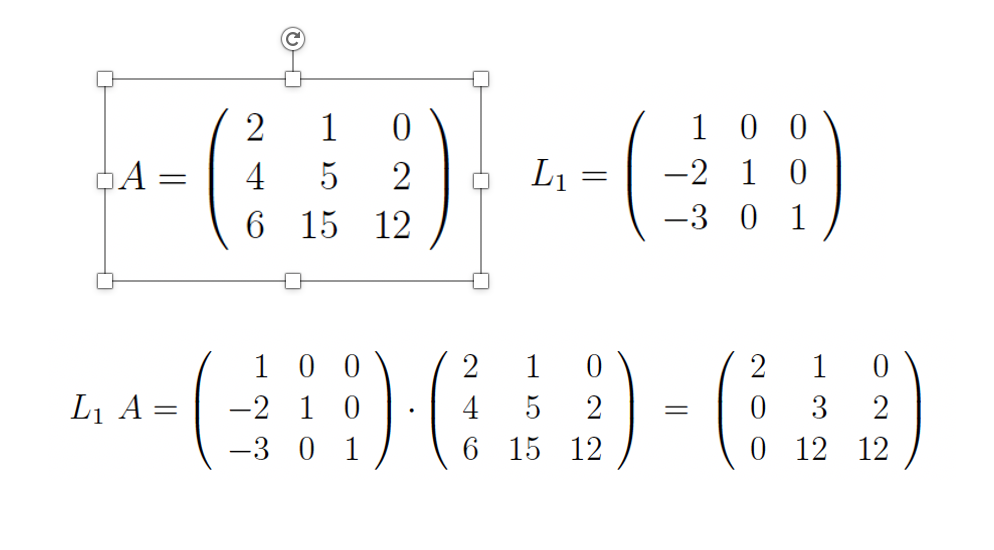
\includegraphics[width=0.7 \textwidth]{sections/lu1.png}

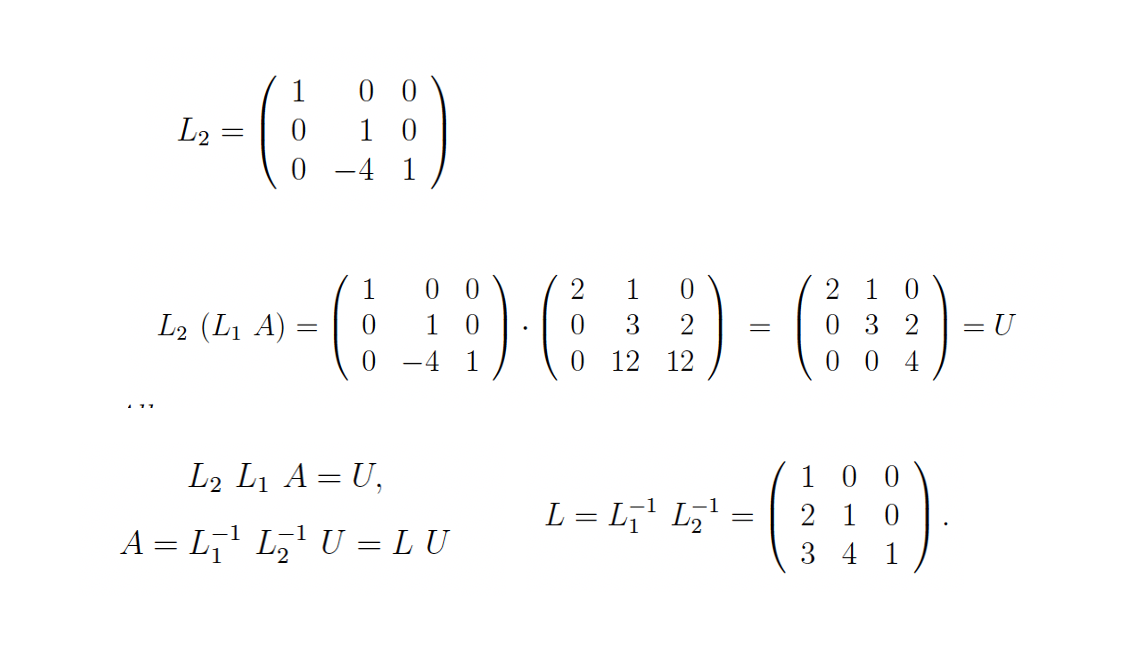
\includegraphics[width=0.8 \textwidth]{sections/lu2.png}

One problem of GEM is that it is \textit{unstable}, i.e. the algorithmic error is not limited. This happens because the elements $a^{(k)}_{kk}$ used to compute the multipliers can be very small or even zero, leading to errors. To avoid this, the \textit{pivoting technique} is employed in order to make the elements $a^{(k)}_{kk}$ as big as possible. This is done by swapping two rows so that $a^{(k)}_{kk}$ is the column element with the maximum absolute value. The swapping can be seen as a left multiplication by a \textit{permutation matrix} $P$, i.e. an identity matrix with the needed rows swapped. 

\textbf{Example}

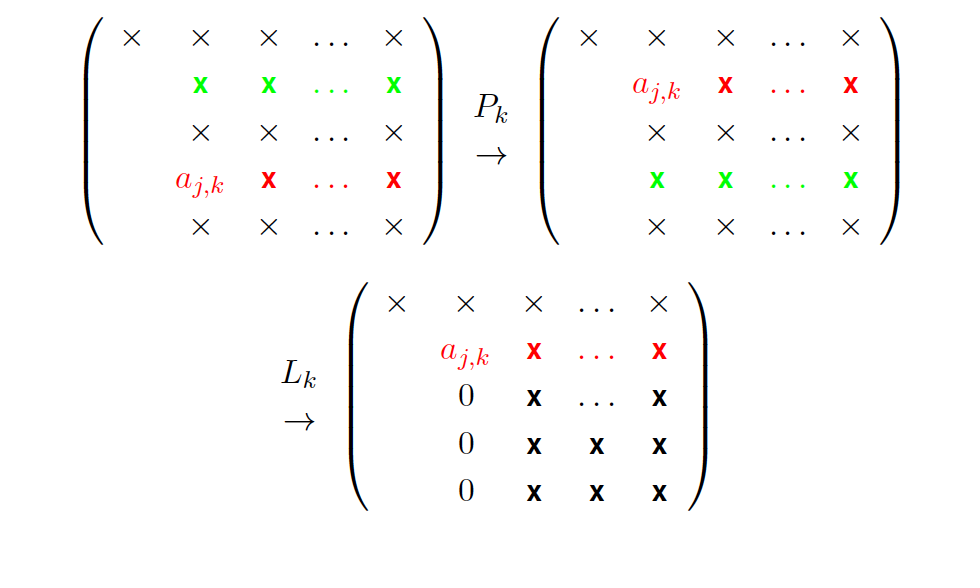
\includegraphics[width=0.7 \textwidth]{sections/images/lup1.png}

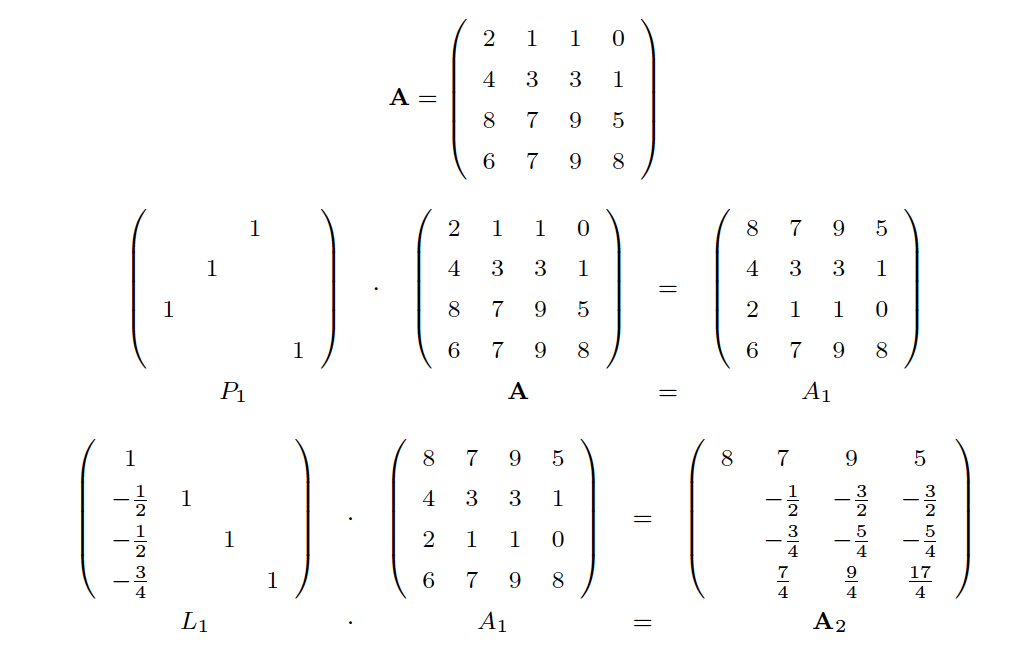
\includegraphics[width=0.8 \textwidth]{sections/images/lup2.png}

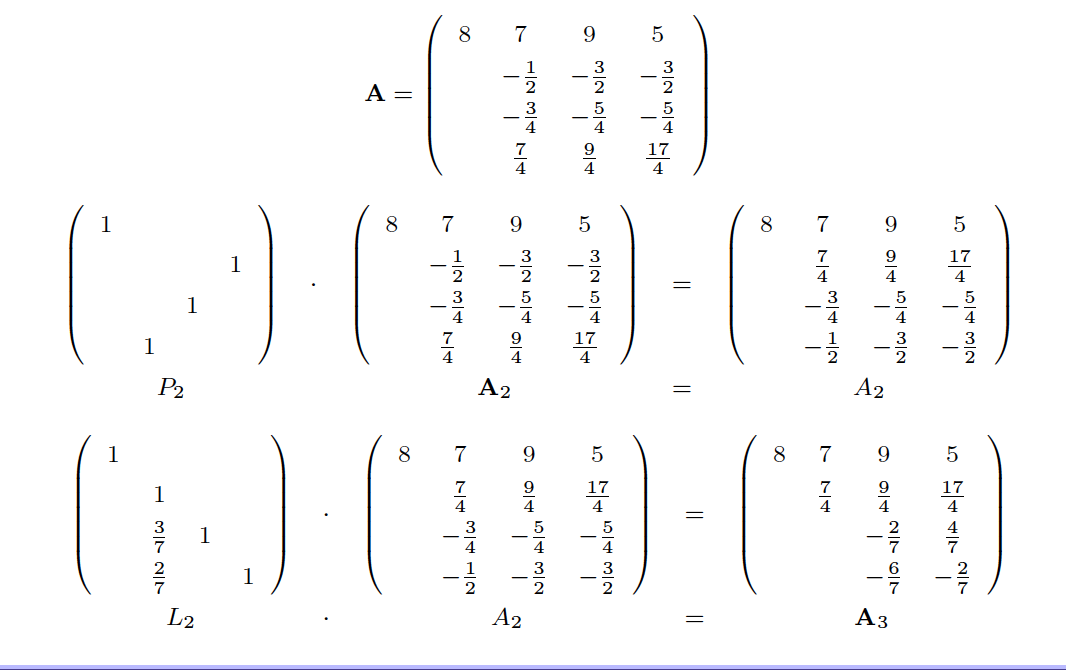
\includegraphics[width=0.8 \textwidth]{sections/images/lup3.png}

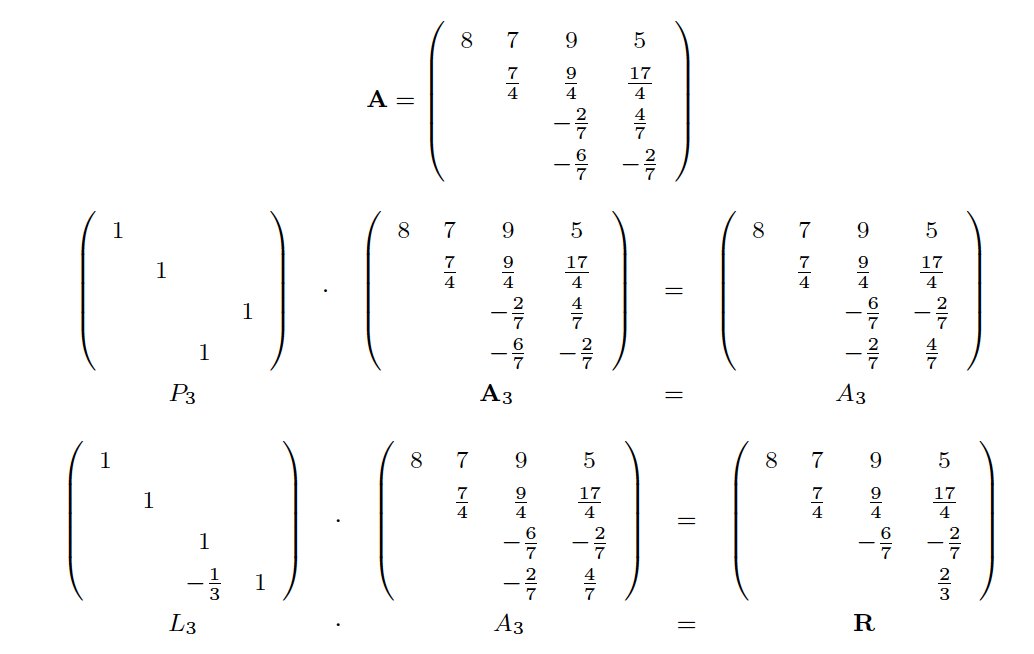
\includegraphics[width=0.8 \textwidth]{sections/images/lup4.png}

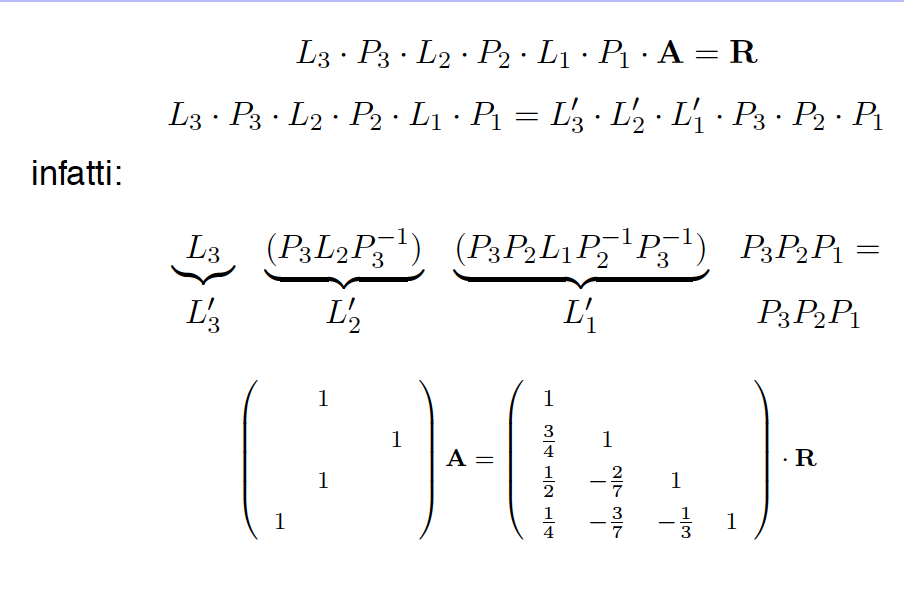
\includegraphics[width=0.8 \textwidth]{sections/images/lup5.png}

% \begin{definition}
%     A matrix $\mat{A} \in \set{R}^{n \times n}$ is positive semi-definite if
%     $$ \forall\vec{x}\in\set{R}^{n},\ \vec{x}\neq\vec{0}\ \ \ \transp{\vec{x}}\mat{A}\vec{x} \geq 0 $$
% \end{definition}

\begin{proposition}
    Let $\mat{A} \in \set{R}^{n \times n}$ be symmetric positive semi-definite. Then it is always possible to $\mat{LU}$-factorize it without using pivoting. In this case we have
    $$ \mat{A} = \mat{L}\transp{L} $$
    
    and the factorization has a computational complexity of $\mathrm{O}(n^3/6)$ (using Cholesky algorithm).
\end{proposition}

\textbf{Example}

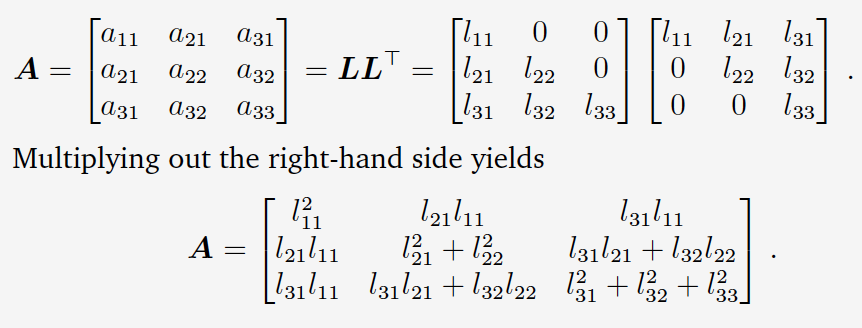
\includegraphics[width=0.7 \textwidth]{sections/images/chol1.png}

The elements $l_{ij}$ of the matrix $\mat{L}$ are computed by comparing the left and roght hand sides of the previous matrix equation.

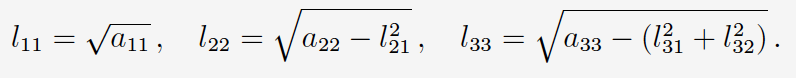
\includegraphics[width=0.8 \textwidth]{sections/images/chol2.png}

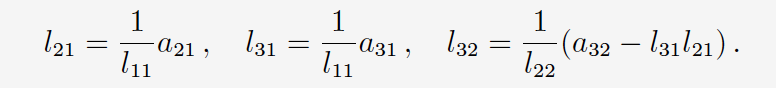
\includegraphics[width=0.8 \textwidth]{sections/images/chol3.png}

The Cholesky decomposition is a very useful tool in numerical linear algebra for Machine Learning, where we often encounter symmetric positive definite matrices. For example, the covariance matrix of a multivariate Gaussian variable
is symmetric positive definite. \\
Moreover, the Cholesky decomposition can be used to efficiently compute the determinant of a symmetric positive definite matrix. We know that $$det(\mat{A})=det(\mat{L}) det(\mat{L^T})=det(\mat{L}^2)=\prod_i l_{ii}^2.$$

\subsection{Singular Value Decomposition (SVD)}

We introduce here a decomposition that involve a diagonal matrix instead of Triangular matrices.

There are mainly two matrix decompositions involving a diagonal matrix: the so called \textit{eigendecomposition} and the \textit{Singular Value Decomposition}.
We will go quickly through the first one and we will analyse in detail the second.

\begin{proposition}
\textit{Eigendecomposition.} Let $\mat{A}$ a square matrix of size $n \times n$. Hence $\mat{A}$ A can be decomnposed as:
$$\mat{A}=\mat{PDP}^{-1}$$
where $\mat{P}$ is a non singular matrix of size $n \times n$ and $\mat{D}$ is a diagonal matrix with diagonal elements $d_{ii}$ corresponding to the eigenvalues of $\mat{A}$ iff the eigenvectors of $\mat{A}$ are linear independent abd form a basis of $]\mathbf{R}^n$.
\end{proposition}

Example 4.11 MML book.

\textbf{Observation.} The eigenvalue decomposition can be applied only to square matrices and with particular properties on their spectrum.

We now introduce the Singulas Value Decomposition (SVD) which can be applied to \textbf{all} the matrices.
We first need some definitions and concepts on \textit{orthogonality}. 

\begin{definition}
    Let $\vec{u}, \vec{v} \in \set{R}^n$. $\vec{u}$ and $\vec{v}$ are \textit{orthogonal} if
    $$ \langle\vec{u}, \vec{v}\rangle = 0 $$
\end{definition}

\begin{definition}
    $\vec{u} \in \set{R}^n$ is a \textit{unit vector} if $\norm{\vec{u}} = 1$.
\end{definition}

\begin{proposition}
    (Normalization) $\forall\vec{u} \in \set{R}^n,\ \ \ \hat{\vec{u}} = \frac{\vec{u}}{\norm{\vec{u}}}$ is a unit vector.
\end{proposition}

\begin{example}
    $$ \vec{u} = [1, 2, 3] $$
    $$ \norm{\vec{u}}_2 = \sqrt{14} $$
    $$ \hat{\vec{u}} = \frac{\vec{u}}{\norm{\vec{u}}} = \left[ \frac{1}{\sqrt{14}}, \frac{2}{\sqrt{14}}, \frac{3}{\sqrt{14}} \right] $$
\end{example}

\begin{definition}
    The set $\{\vec{u}_1, \vec{u}_2, \hdots, \vec{u}_p\},\ \vec{u}_i \in \set{R}^n,\ i = 1, \hdots, p$ is an \textit{orthogonal set} if $\langle\vec{u}_i, \vec{u}_j\rangle = \transp{\vec{u}_i}\vec{u}_j = 0,\ \forall i \neq j$
\end{definition}

\begin{example}
    $$ \vec{u}_1 = \transp{[3, 1, 1]},\ \vec{u}_2 = \transp{[-1, 2, 1]},\ \vec{u}_3 = \transp{\left[ -\frac{1}{2}, -2, \frac{7}{2} \right]} $$
    is an orthogonal set because
    $$ \langle\vec{u}_1, \vec{u}_2\rangle = 0,\ \langle\vec{u}_1, \vec{u}_3\rangle = 0,\ \langle\vec{u}_2, \vec{u}_3\rangle = 0,\  $$
\end{example}

\begin{proposition}
    If $\vec{u}_1, \vec{u}_2, \hdots, \vec{u}_p \in \set{R}^n$ are orthogonal then they are linearly independent. The set $\{\vec{u}_1, \vec{u}_2, \hdots, \vec{u}_p\},\ \vec{u}_i \in \set{R}^n,\ i = 1, \hdots, p$ is an \textit{orthogonal basis} for $U = \text{span}\{\vec{u}_1, \vec{u}_2, \hdots, \vec{u}_p\}$.
\end{proposition}

\begin{definition}
    The set $\{\vec{u}_1, \vec{u}_2, \hdots, \vec{u}_p\},\ \vec{u}_i \in \set{R}^n,\ i = 1, \hdots, p$ is an \textit{orthonormal set} if it is an orthogonal set of unit vectors. A basis of orthonormal vectors is called \textit{orthonormal basis}.
\end{definition}

\begin{definition}
    Let $\mat{U} \in \set{R}^{m \times n}$. $\mat{U}$ is an \textit{orthogonal matrix} iff $\transp{U}\mat{U} = \mat{I}$. If $m = n$ then $\transp{U} = \inv{U}$.
\end{definition}

\begin{proposition}
    If $\mat{U}^{m \times n}$ is orthogonal then
    
    \begin{itemize}
        \item $\norm{\mat{U}\vec{x}}_2 = \norm{\vec{x}}_2,\ \forall\vec{x} \in \set{R}^n$
        \item $\langle\mat{U}\vec{x}, \mat{U}\vec{y}\rangle = \langle\vec{x}, \vec{y}\rangle,\ \forall\vec{x}, \vec{y} \in \set{R}^n$
        \item $\langle\mat{U}\vec{x}, \mat{U}\vec{y}\rangle = 0 \iff \langle\vec{x}, \vec{y}\rangle = 0,\ \forall\vec{x}, \vec{y} \in \set{R}^n$
    \end{itemize}
\end{proposition}

Transformations by orthogonal matrices preserve both length and angles.

We present the SVD in the case $m ]\geq n$ but it can be easily extended to the case $m<n$ (see for example MML book).
\begin{proposition}
\textit{singular value decomposition} (SVD).
Any matrix $\mat{A} \in \set{R}^{m \times n},\ m \geq n$ with $\rank{A} = k,\ k \leq n$ can be written as
$$ \mat{A} = \mat{U}\mat{\Sigma}\transp{V} $$
where
\begin{itemize}
    \item $\mat{U} \in \set{R}^{m \times m}$ is an orthogonal matrix with orthogonal vectors $\vec{u}_i$
    \item $\mat{V} \in \set{R}^{n \times n}$ is an orthogonal matrix with orthogonal vectors $\vec{v}_i$
    \item $\Sigma \in \set{R}^{m \times n}$ is a matrix whose diagonal entries are the \textit{singular values} $\sigma_i$ of $\mat{A}$ and with extra-diagonal entries equal to 0.
\end{itemize}
\end{proposition}

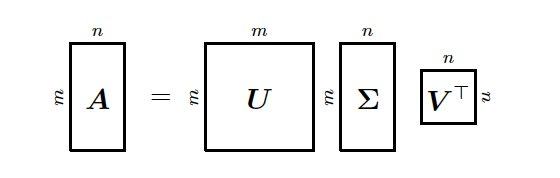
\includegraphics[width=0.7 \textwidth]{sections/images/svd.png}

 The singular values enjoy the following property
    $$ \sigma_1 \geq \sigma_2 \geq \hdots \geq \sigma_k > \sigma_{k+1} = \sigma_{k+2} = \hdots = \sigma_{n} = 0 $$
    where $k = \rank{A}$. The singular matrix $\Sigma$ is unique, while the orthogonal matrices $\mat{U}$ and $\mat{V}$ aren't.

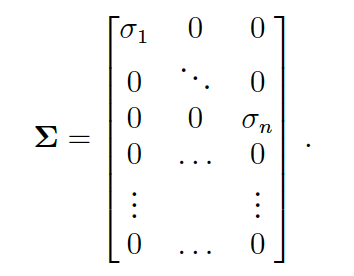
\includegraphics[width=0.5 \textwidth]{sections/images/svd1.png}

From the geometric point of view, the SVD performs two changes of basis, via the orthogonal matrices $\mat{U}$ and $\mat{V}$ and a scaling operation via the matrix $\Sigma$. The columns of $\mat{U}$ and $\mat{V}$ are sets of orthonormal basis of $\mathbf{R}^m$ and $\mathbf{R}^n$, respectively. See Example 4.12 MML book, page 121.

\textit{Results}
\begin{itemize}
\item Since the following relation holds:
$$\mat{A}\vec{v}_i=\sigma_i \vec{u}_i,\ i = 1, \ldots, n$$
$\vec{v}_i$ are called \textit{right singular vectors} and $\vec{u}_i$ are called \textit{left singular vectors}.
\item 
We have the following relation between the singular values of $\mat{A}$ and the eigenvalues of $\mat{A^T A}$.
$$\mat{A^T A}=(\mat{U \Sigma V^T})^T(\mat{U \Sigma V^T})=\mat{V \Sigma ^T U^T U \Sigma V^T}$$
Hence 
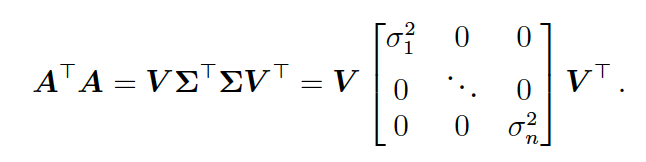
\includegraphics[width=0.7 \textwidth]{sections/images/svd2.png}

and
$$\sigma_i = \sqrt{\lambda_i(\transp{A}\mat{A})},\ i = 1, \hdots, n$$
In particular:
$$ \sigma_1 = \sqrt{\lambda_{max}(\transp{A}\mat{A})} = \sqrt{\rho(\transp{A}\mat{A})} = \norm{A}_2 $$
$$ \sigma_n = \sqrt{\lambda_{min}(\transp{A}\mat{A})} \implies \norm{\inv{A}}_2 = \frac{1}{\sigma_n} $$
Thus,
$$ K(\mat{A}) = \frac{\sigma_1}{\sigma_2} $$
\item The right singular vectors of $\mat{A}$ are the eigenvectors of $\mat{A^T A}$
\item The left singular vectors of $\mat{A}$ are the eigenvectors of $\mat{AA^T }$
\item For symmetric matrices $\mat{A}$ the eigenvalue decomposition and the SVD are one and the same.

\end{itemize}

\textit{Moore-Penrose inverse}.
The SVD can be used to compute the \textit{Moore-Penrose inverse} (or simply \textit{pseudoinverse}) of a matrix $\mat{A} \in \set{R}^{m \times n}$
$$ \mat{A}^{+} = \mat{V}\Sigma^{+}\transp{U} $$
where $\Sigma^{+} \in \set{R}^{n \times m}$ is the pseudoinverse of $\Sigma$, computed by taking the reciprocal of every non-zero diagonal element, leaving the zeros in place and transposing the matrix
$$
    \Sigma =
    \begin{bmatrix}
        \sigma_1 & 0 & \hdots & 0\\
        0 & \sigma_2 & \hdots & 0\\
        0 & 0 & \ddots & 0\\
        0 & 0 & 0 & \sigma_n\\
        0 & 0 & 0 & 0\\
        \vdots & \vdots & \vdots & \vdots\\
        0 & 0 & 0 & 0
    \end{bmatrix},\ \ \ \ 
    \Sigma^{+} =
    \begin{bmatrix}
        \frac{1}{\sigma_1} & 0 & \hdots & 0 & \hdots & 0\\
        0 & \frac{1}{\sigma_2} & \hdots & 0 & \hdots & 0\\
        0 & 0 & \ddots & 0 & \hdots & 0\\
        0 & 0 & 0 & \frac{1}{\sigma_n} & \hdots & 0\\
    \end{bmatrix}
$$


\subsection{Matrix approximation using SVD}
Given the SVD of a matrix $\mat{A} \in \set{R}^{m \times n}$
$$ \mat{A} = \mat{U}\Sigma\transp{V} $$
we can use it to represent (or approximate) the matrix $\mat{A}$ as a sum of low-rank matrices $\mat{A}_i \in \set{R}^{m \times n}$ with $\text{rank}(\mat{A}_i) = 1$ such that
$$ \mat{A}_i = \vec{u}_i\transp{\vec{v}_i} $$
The matrix $ \mat{A}$ of $\rank{A} = k$ can then be written as
$$ \mat{A} = \sum^{k}_{i = 1}{\sigma_i\mat{A}_i} = \sum^{k}_{i = 1}{\sigma_i\vec{u}_i\transp{\vec{v}_i}} $$

To obtain a rank-$p$ approximation $\mat{A}_p$ ($p < k$) of $\mat{A}$ we can truncate the sum at index $i = p$. The error introduced with this approximation can be computed as
$$ \norm{\mat{A} - \mat{A}_p}_2 = \left|\left|\sum^{k}_{i = p+1}{\sigma_i\mat{A}_i}\right|\right|_2 = \sigma_{p+1}$$
This means that if $\sigma_{p+1}$ is small we have a good approximation of the original matrix $\mat{A}$.

\begin{theorem}
    Given $\mat{A} \in \set{R}^{m \times n},\ \rank{A} = k$, let $\mat{A} = \mat{U}\Sigma\transp{V}$ be its singular value decomposition. Let $\mat{A}_p = \sum^{p}_{i = 1}{\sigma_i\vec{u}_i\transp{\vec{v}_i}}$ be the rank-$p$ approximation of $\mat{A}$. Then
    $$ \forall \mat{B} \in \set{R}^{m \times n},\ \rank{B} = p,\ \norm{\mat{A} - \mat{A}_p}_2 \leq \norm{\mat{A} - \mat{B}}_2 $$
    So $\mat{A}_p$ is the best rank-$p$ approximation of $\mat{A}$ obtained via singular value decomposition.
\end{theorem}

Example. \textit{Rank-p approximation of an image matrix}.

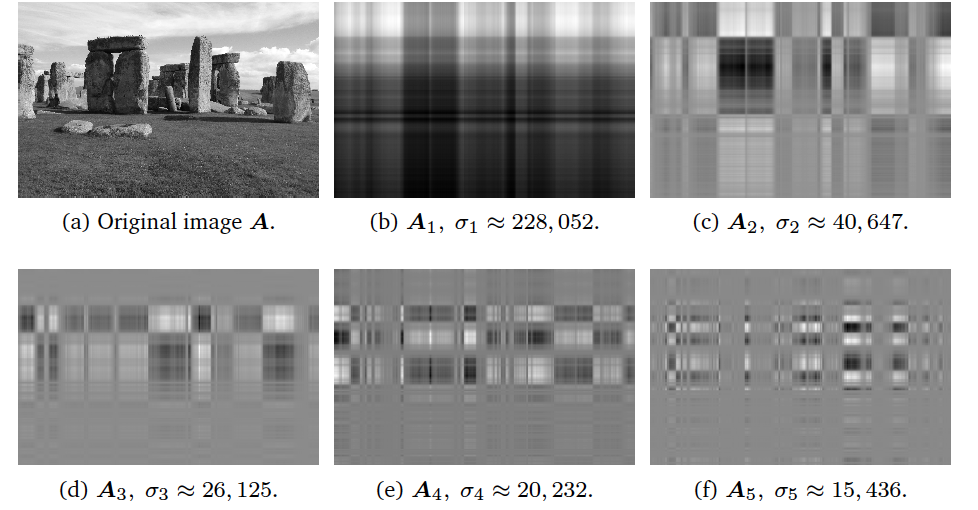
\includegraphics[width=0.7 \textwidth]{sections/images/svd3.png}

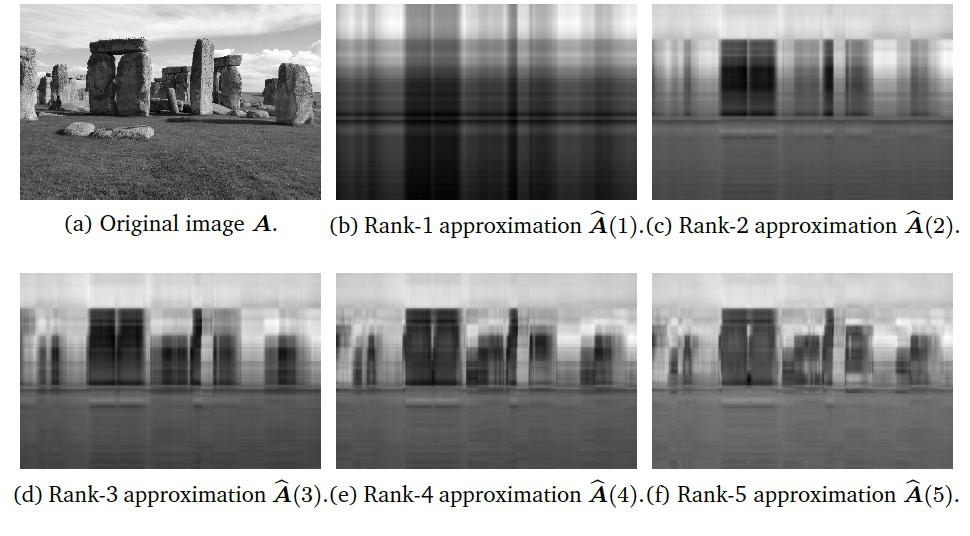
\includegraphics[width=0.7 \textwidth]{sections/images/svd4.png}

The matrix associated to the original image has size $m \times n=1432 \times 1910$, hence it requires 2735120 data. If we consider the rank-p approximation ,it requires $(m+n+1)\times p$ data. For example, the rank-5 approximation requires $5\times(1432+1910+1)=16715$ data, corresponding to about $0.6 \%$ of the original one.
Hence we can interpret the rank-p SVD approximation of a matrix $\mat{A}$ as a lossy compression. This approximation appears in different machine learning applications, such as image processing, noise filtering and regularization of ill-posed problems. Moreover, it is a fundamental tool in the PCA analysis.

We can see the rank-p approximation obtain through SVD as the projection of $\mat{A}$ onto a subspace of matrices of rank p. Among all the possible projections, rank-p SVD approximation minimizes the error in the 2-norm betweeen $\mat{A}$ and any rank-p approximation of $\mat{A}$.

Examples 4.14 and 4.15 MML book \textit{finding structure in Movie Ratings and Customers}

\subsection{Conclusions}

We can summarize many tools and ideas in the following figure, where we can see the relationship between different types of matrices.

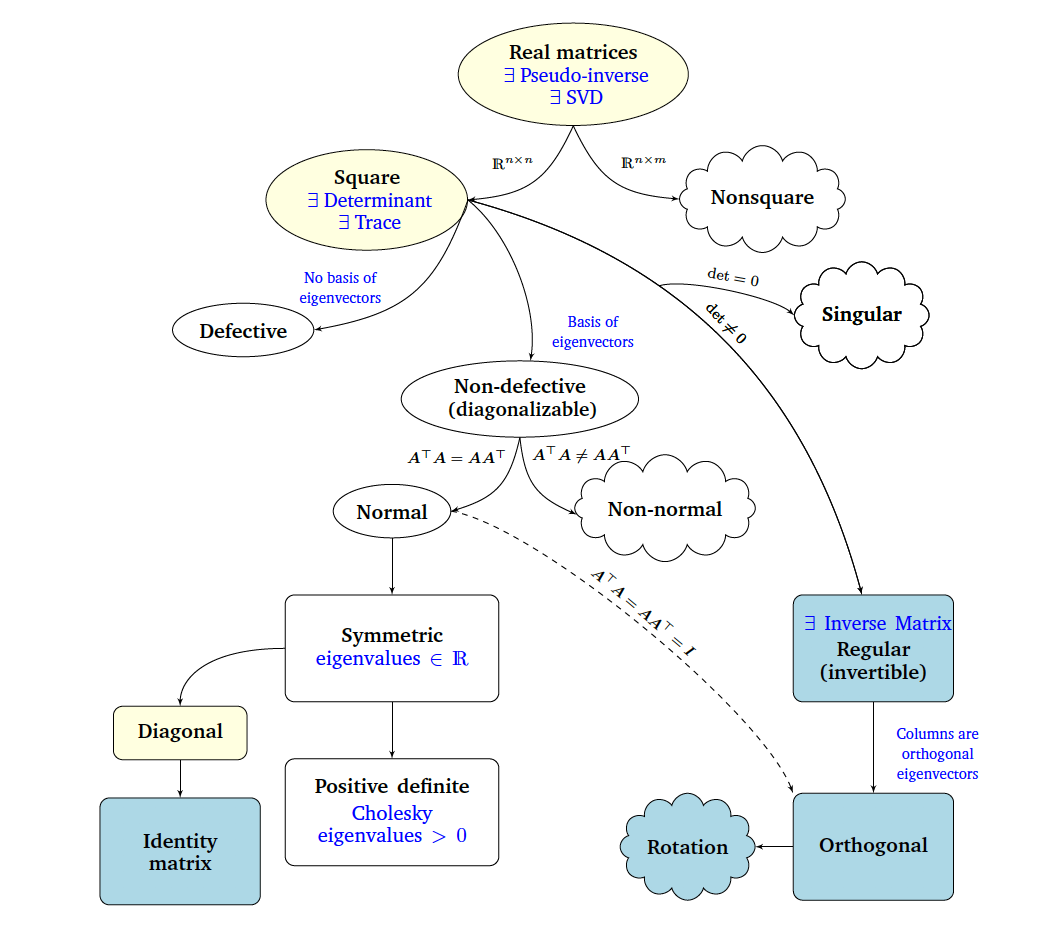
\includegraphics[width=0.7 \textwidth]{sections/images/matrix.png}

 \section{Linear systems \label{sec:syslin}}
 \subsection{Introduction to linear systems}

A linear system can be written as
$$ \mat{A}\vec{x} = \vec{b} $$
where $\mat{A}$ is a matrix of size $m \times n$ (we suppose $m \geq n$) and $\vec{x}$ is a coulumn vector of length $n$ and $\vec{b}$ is a column vectors of length $m$. $\vec{x}$ represents the unknown solution while $\vec{b}$ is a given vector. This form can be expanded as
$$
    \begin{matrix}
        a_{11}x_1 + a_{12}x_2 + \hdots + a_{1n}x_n = b_1\\
        a_{21}x_1 + a_{22}x_2 + \hdots + a_{2n}x_n = b_2\\
        \vdots\\
        a_{m1}x_1 + a_{m2}x_2 + \hdots + a_{mn}x_n = b_m
    \end{matrix}
$$

We are interested in:

\begin{itemize}
    \item Existence and uniqueness of a solution
    \item Numerical methods to find the solution
    \item Conditioning of the problem
\end{itemize}

We separately consider the case of square linear systems ($m=n$) and least squares problem ($m>n$).

\subsection{Square linear systems}


\begin{proposition}
    The solution of a linear system
    $$ \mat{A}\vec{x} = \vec{b} $$
    with $\mat{A}$ of dimension $n \times n$, $\vec{x}$ and $\vec{b}$ of dimension $n$ exists and is unique iff one of the following conditions holds:
    
    \begin{itemize}
        \item $\mat{A}$ is non-singular
        \item $\rank{A} = n$
           \item The system $\mat{A}\vec{x} = \vec{0}$ admits only the solution $\vec{x} = \vec{0}$
    \end{itemize}

\end{proposition}

The solution can be algebraically computed in the following way
$$ \mat{A}\vec{x} = \vec{b} \implies \inv{A}\mat{A}\vec{x} = \inv{A}\vec{b} \implies \vec{x} = \inv{A}\vec{b} $$
The problem with this kind of method is that computing the inverse of $\mat{A}$ can be expensive for large values of $n$.

Another method to compute the solution of a system is \textit{Cramer's rule}:
$$ x_i = \frac{\det{A_i}}{\det{A}},\ i = 1, \hdots, n $$
where $\mat{A}_i$ is obtained from $\mat{A}$ by replacing the $i$-th column by $\vec{b}$

As for the previous one, the computation of determinants can be quite expensive for large values of $n$.

We will consider two different approaches to find the solution of a linear system:

\begin{itemize}
    \item \textit{direct methods}. They yield the solution in a finite number of steps; they are more precise but more expensive in terms of computational cost
    \item \textit{iterative methods}. They require (in principle) an infinite number of steps; they are less precise and less expensive
\end{itemize}

It is very important to also perform an error analysis on the obtained results. It generally includes two parts:
\begin{itemize}
    \item \em{Rounding} or \em{arithmetic errors}. They depend on the algorithm steps. An algorithm producing an arithmetic error limited by a constant is called a \textbf{stable algorithm}.
    \item \textit{Inherent errors}. They are due to the errors in the data representation and the DO NOT depend on the algorithm. For this reason, if the inherent error is large,we speak about \textbf{ill-posed problem}.
\end{itemize}

\subsection{Direct methods}

In the case of direct methods we factorize the matrix A as in section \ref{sec:matdecomp}.
Let $\mat{A}=\mat{L} \mat{U}$, then 
 the solution of the linear system $\mat{A}\vec{x} = \vec{b}$ can be computed by solving two triangular systems
$$
    \begin{matrix}
        \mat{L}\vec{y} = \vec{b}\ \text{(forward substitutions algorithm)}\\
        \mat{U}\vec{x} = \vec{y}\ \text{(backward substitutions algorithm)}
    \end{matrix}
$$

\textbf{Forward substitution.}

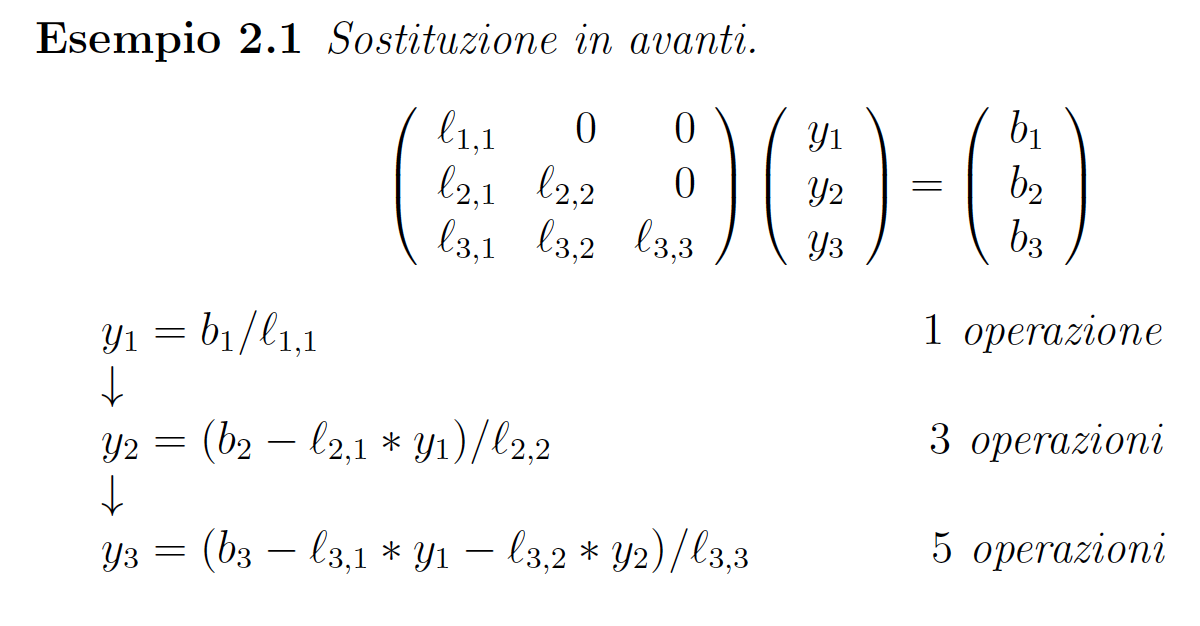
\includegraphics[width=0.7 \textwidth]{sections/images/forsub.png}

\textbf{Backward substitution.}

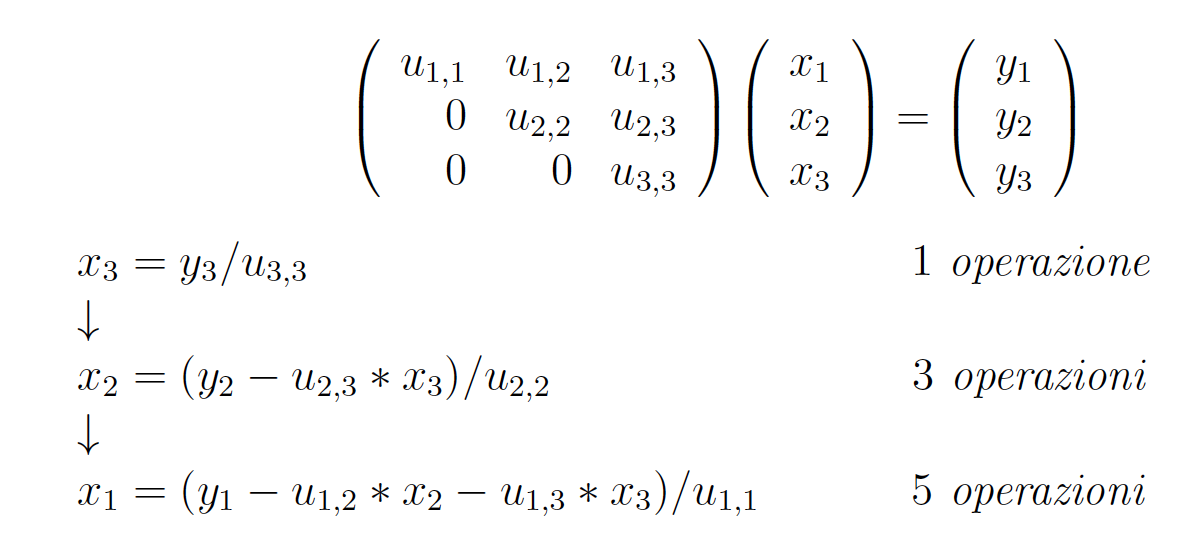
\includegraphics[width=0.7 \textwidth]{sections/images/backsub.png}

In the case of pivoting algorithm, we have that $\mat{P} \mat{A}=\mat{L} \mat{U}$. Then 
 the solution of the linear system $\mat{P} \mat{A}\vec{x} = \mat{P} \vec{b}$ can be computed by solving two triangular systems
$$
    \begin{matrix}
        \mat{L}\vec{y} = \mat{P}\vec{b}\ \text{(forward substitutions algorithm)}\\
        \mat{U}\vec{x} = \vec{y}\ \text{(backward substitutions algorithm)}
    \end{matrix}
$$

\subsection{Iterative methods}

Iterative methods are numerical methods that approximate a solution using a procedure involving several (or an infinite amount of) steps. 
%Each iteration requires $n^2$ multiplications, meaning that these methods have a computational cost of $\mathrm{O}(n^2)$.

The basic idea of iterative methods is to construct a sequence of vectors $\vec{x}_k$ enjoying the property of \textit{convergence}
$$ \vec{x}^* = \lim_{k \rightarrow \inf}{\vec{x}_k} $$
where $\vec{x}^*$ is the exact solution and the starting guess $\vec{x}_0$ is given.

In general the sequence $\vec{x}_k$ is obtained as $\vec{x}_k=g(\vec{x}_{k-1}), \ k=1,\ldots$ where $g$ is a particular function or set of operations acting on $\vec{x}_{k-1}$.
Different classes of iterative methods are defined for different expressions of $g$.
In general, an iterative method converges for matrices with fixed properties (such as on the shape, on the eigenvalues, ...).

Iterative methods are sensitive to both algorithmic and truncation errors.

Examples of iterative methods (the most common):

\begin{itemize}
    \item \textit{stationary iterative methods}, they take the form
    $$\vec{x}_{k+1} = \mat{B}\vec{x}_k + \vec{f}$$
    where $\mat{B}$ is called \textit{iteration matrix} and $\vec{f}$ is a vector obtained from $\vec{b}$
    \item \textit{gradient-like methods}, they take the form
    $$\vec{x}_{k+1} = \vec{x}_k + \alpha_k\vec{p}_k$$
    where $\alpha_k \in \set{R}$, $\vec{p}_k$ is a vector called \textit{direction}.
    
    If $\mat{A}$ is symmetric and positive definite and the vectors $\vec{p_k}$ have the \textit{conjugacy} property, i.e:
    $$\vec{p}_i^T\mat{A}\vec{p}_k=0 \ \ if \ i \neq k $$
    then the method is called \textit{Conjugate Gradients}.
\end{itemize}

All these methods require one matrix-vector multiplication per iteration. Hence, if $\mat{A}$ is a \textit{full} matrix the computational complexity is $O(n^2)$ per iteration.

Stopping criteria for iterative methods for linear systems are:
\begin{itemize}
\item defined the residual $\vec{r}_k=\bb-\AAA\xx_k$ at iteration $k$, stop the algorithm when
\begin{itemize}
   \item $\|\vec{r}_k\| \le \epsilon$ (absolute criterion)
    \item $\frac{\|\vec{r}_k\|}{\|\bb\|} \le \epsilon$ (relative criterion)
    \end{itemize}
    \item $\|\vec{x}_{k+1}-\vec{x}_k\| \le \tau$ (absolute criterion)
\end{itemize}

\textbf{Sparse matrices}
A matrix $\mat{A}$ is called \textit{sparse} if it has a very small percentage (i.e. $0.05-0.06 \%$ ) of non-null elements. In this case, the matrix is not fully stored, but only the non-null elements and their indices are stored. The matrix-vector multiplication requires $k$ multiplications, where $k$ is the number of non-null elements.


\subsection{Inherent errors in linear systems}
WE remind that inherent errors are due to the errors in the data representation. They \textbf{do not} depend on the algorithm used for computing the result. Really, the analysis of inherent errors is performed by supposing to use exact arithmetic to compute the result. 

Consider now a linear system $\mat{A}\vec{x} = \vec{b}$. What happens to the solution $\vec{x}$ when $\mat{A}$ and/or $\vec{b}$ slightly change (e.g. due to machine precision)?

Suppose that $\mat{A}$ doesn't change while $\vec{b}$ changes in $\vec{b} + \Delta\vec{b}$. The linear system becomes
$$ \mat{A}(\vec{x} + \Delta\vec{x}) = \vec{b} + \Delta\vec{b},\ \Delta\vec{x}\ \text{inherent error} $$

We want to compare $\left|\left|\frac{\Delta\vec{x}}{\vec{x}}\right|\right|$ and $\left|\left|\frac{\Delta\vec{b}}{\vec{b}}\right|\right|$ to see how much the solution has changed with respect to $\vec{b}$. Let's subtract $\mat{A}\vec{x} = \vec{b}$ to $\mat{A}(\vec{x} + \Delta\vec{x}) = \vec{b} + \Delta\vec{b}$
$$ \mat{A}\Delta\vec{x} = \Delta\vec{b} \implies \Delta\vec{x} = \inv{A}\Delta\vec{b} $$
Then we have
$$ \norm{\Delta\vec{x}} = \norm{\inv{A}\Delta\vec{b}} \leq \norm{\inv{A}}\ \norm{\Delta\vec{b}} $$
and from the linear system equation
$$ \norm{\mat{A}\vec{x}} = \norm{\vec{b}} \implies \norm{\vec{b}} = \norm{\mat{A}\vec{x}} \leq \norm{\mat{A}}\ \norm{\vec{x}} \implies \norm{\vec{x}} \geq \left|\left|\frac{\vec{b}}{\mat{A}}\right|\right| $$
Thus we have
$$ \left|\left|\frac{\Delta\vec{x}}{\vec{x}}\right|\right| \leq \norm{\inv{A}} \cdot \norm{\mat{A}} \cdot \frac{\norm{\Delta\vec{b}}}{\norm{\vec{b}}} = K(\mat{A)}\frac{\norm{\Delta\vec{b}}}{\norm{\vec{b}}} $$
\begin{definition}
    The \textit{condition number} of a matrix $\mat{A} \in \set{C}^{n \times n}$ is defined as
    $$ K(\mat{A}) = \norm{\mat{A}}\ \norm{\inv{A}} $$
    where $\norm{\cdot}$ is a matrix norm. In general $K(\mat{A})$ depends on the choice of the norm, indicated by a subscript.
\end{definition}
Notice that $K(\mat{A}) \geq 1$ since
$$ 1 = \norm{\mat{A}\inv{A}} \leq \norm{\mat{A}}\ \norm{\inv{A}} = K(\mat{A}) $$

The condition number measures how sensitive a function is to changes/errors in the input and how much the output changes as a result of the operations performed. A \textit{well-conditioned} system is a system where $K(\mat{A})$ is small, while an \textit{ill-conditioned} system is a system where $K(\mat{A})$ is large.

If $K(\mat{A})$ is very large, the matrix $\mat{A}$ is near (with respect to a norm) a singular matrix and its columns are quasi-linearly dependent. Regularization techniques can be used in order to reduce $K(\mat{A})$.

\begin{example}
    The condition number for p-norm with $p = 2$ is
    $$
        \begin{matrix}
            \norm{\mat{A}}_2 = \sqrt{\rho(\transp{A}\mat{A})} = \lambda_{max}\\
            \norm{\inv{A}}_2 = \frac{1}{\sqrt{\rho(\transp{A}\mat{A})}} = \frac{1}{\lambda_{min}}\\
            K_2(\mat{A}) = \norm{\mat{A}}\ \norm{\inv{A}} = \frac{\lambda_{max}}{\lambda_{min}}
        \end{matrix}
    $$
    where $\lambda_{max}$ and $\lambda_{min}$ are the maximum and minimum eigenvalues of $\mat{A}$
\end{example}

\subsection{Linear least squares}

Consider an \textit{overdetermined system}
$$ \mat{A}\vec{x} = \vec{b} $$
where $\mat{A}$ has dimension $m \times n$ with $m > n$, $\vec{x}$ of dimension $n$ and $\vec{b}$ of dimension $m$. Such a system usually has no solution, meaning that $\vec{b}$ does not lie on the subspace spanned by the columns of $\mat{A}$ (denoted by $\text{Col}(\mat{A})$ from now on). Since no exact solution exists for this problem, we would like to compute the best approximate solution.
We need some tools.

\subsubsection{Orthogonality and projections}

Projections are an important class of linear transformations. In machine learning one often deals with high-dimensional data which is hard to visualize and analyze. Oftentimes, only a few dimensions contain useful information, meaning that other dimensions are not essential to understanding the data. When applying data compression techniques we want to minimize the loss of information by finding the most informative dimensions of the data first.

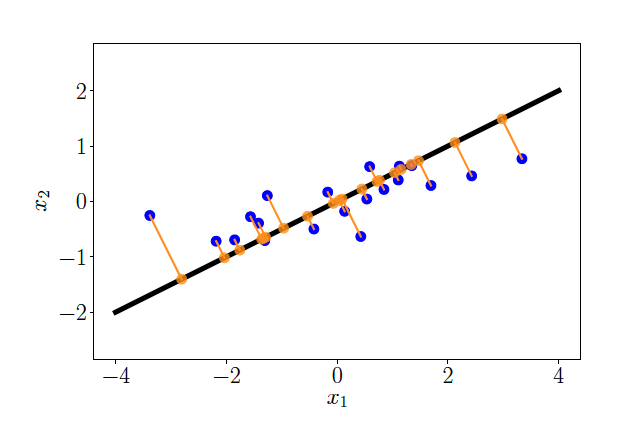
\includegraphics[width=0.7 \textwidth]{sections/images/orth1.png}

\textbf{Orthogonal projection onto a subspace of dimension 1.} 

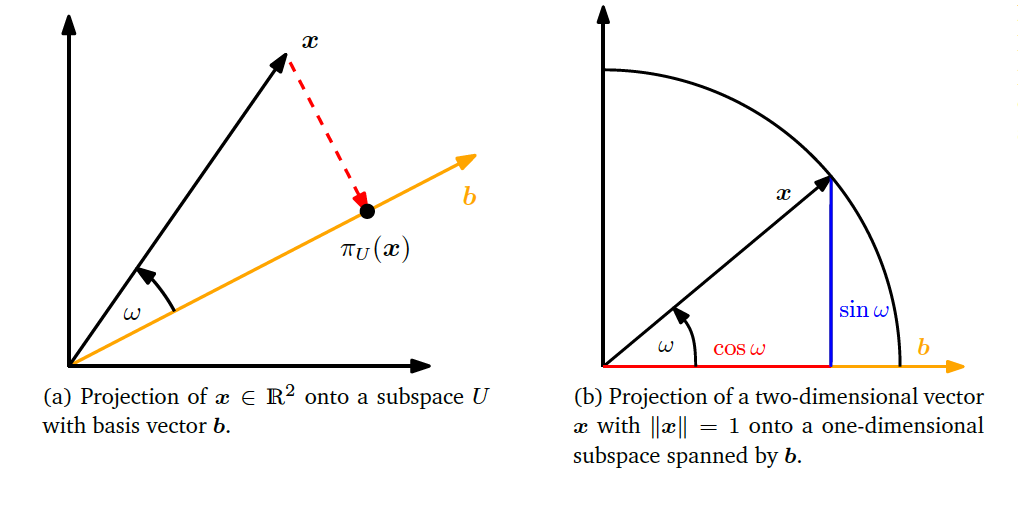
\includegraphics[width=0.7 \textwidth]{sections/images/orth2.png}

\begin{itemize}
    \item The projection $z=\Pi_U(\vec{x})$ is the closest point to $\vec{x}$ of the subspace $U$ generated by $\vec{b}$ by considering as the measure of the distance the 2-norm ($\| \cdot \|_2$). The vector $\zz -\xx$ (the red dashed one in the figure) is orthogonal to the subspace $U$ (and to the vector $\bb$ generating $U$). Hence, the scalar product: $<\vec{z}-\vec{x},\vec{b}>=0$
    \item The vector $\vec{z}$ is a vector of the subspace generated by $\vec{b}$, hence $\vec{z}=\alpha \vec{b}$, $\alpha \in \mathbf{R}.$
  
\end{itemize}


%\begin{example} (In 2 dimensions)\\
    % Let $\vec{y} \in \set{R}^2$ and $L=\text{span}\{\vec{u}\}$ one-dimensional subspace of $\set{R}^2$ generated by $\vec{u} \in \set{R}^2$. We can write $\vec{y}$ as
    % $$ \vec{y} = \hat{\vec{y}} + \vec{z} $$
    % and notice that $\vec{u} \parallel \hat{\vec{y}}$.
    
    % The projection $\hat{\vec{y}}$ is the closest vector lying in the subspace $L$ to $\vec{y}$, where distance is measured by $\norm{\vec{y} - \hat{\vec{y}}}$. It follows that $\vec{z} = \vec{y} - \hat{\vec{y}}$ is orthogonal to $L$ and, in particular, to $\vec{u}$, i.e. $\langle\vec{z}, \vec{u}\rangle = 0$.
    
   % Since $\hat{\vec{y}}$ is an element of $L$ it is a multiple of $\vec{u}$
    %$$ \hat{\vec{y}} = \alpha\vec{u} $$
    
    We can find $\alpha$ in the following way
    $$ \langle\vec{x} - \zz, \vec{b}\rangle = 0 \implies \langle\vec{z} - \alpha\vec{x}, \vec{b}\rangle = 0 \implies \langle\vec{x}, \vec{b}\rangle - \alpha\langle\vec{b}, \vec{b}\rangle = 0 $$
    $$ \alpha = \frac{\langle\vec{x}, \vec{b}\rangle}{\langle\vec{b}, \vec{b}\rangle} = \frac{\transp{\vec{x}}\vec{b}}{\norm{\vec{b}}^2} $$
%\end{example}

Example when projecting from $\mathbf{R}^3$ to $\mathbf{R}^2$.

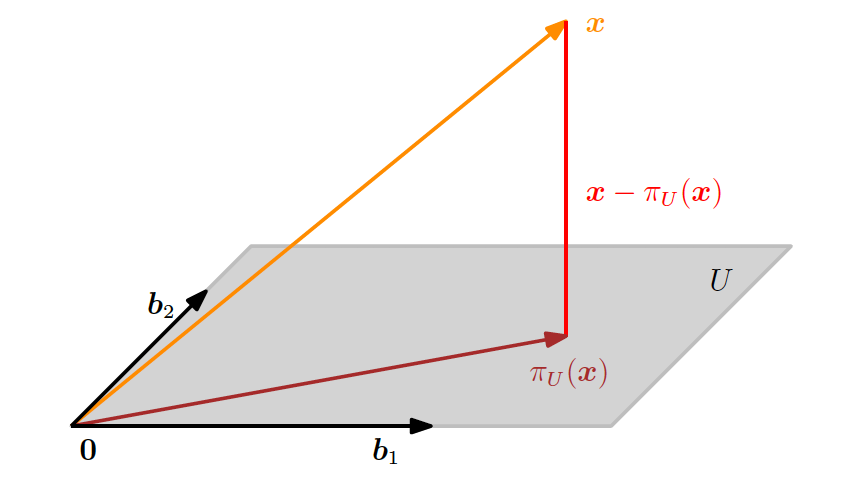
\includegraphics[width=0.7 \textwidth]{sections/images/orth3.png}

We now generalize to sub-spaces of dimension possibly greater than one.

\begin{theorem} (Best approximation theorem)
    Let $W$ a subspace with dimension $p$ of $\set{R}^n$, $\vec{y} \in \set{R}^n$ and $\hat{\vec{y}} = \mathrm{proj}_W(\vec{y})$. Then $\norm{\vec{y} - \hat{\vec{y}}} < \norm{\vec{y} - \vec{v}},\ \forall \vec{v} \in W,\ \vec{v} \neq \hat{\vec{y}}$.
\end{theorem}

This means that $\hat{\vec{y}}$ is the best approximation of $\vec{y}$ in $W$.

Example 3.10 MML book.

The idea is to use projections to find the vector in $\text{Col}(\mat{A})$ (i.e. the subspace generated by set of all the columns of $\AAA$) which is closest to $\vec{b}$. As already seen in the previous chapter, this vector is indeed the orthogonal projection of $\vec{b}$ onto the subspace $\text{Col}(\mat{A})$.

\subsubsection{The linear least squares problem}

When $\AAA$ has size $m \times n$ with $m>n$, it is not possible to find a solution of the linear system $\AAA \xx=\bb$.
The orthogonal projections allow to find a vector $\xx$ that is \textit{near} the system solution (in the sense of the 2-norm).

The problems is then formulated as to compute 
 $\hat{\xx}$ so that:
\begin{equation}
   \hat{\xx}= argmin_x \|\AAA \xx-\bb\|_2^2
   \label{llsq}
\end{equation}

For what concerns existence and uniqueness of the solution of the linear least squares problem, 
two different cases are possible:

\begin{itemize}
    \item $\rank{A} = n$, meaning that every column of $\mat{A}$ is linearly independent. A unique solution exists $\forall \vec{b} \in \set{R}^m$. Let $\vec{x^{*}}$ be the approximate solution to the linear system, we have
    $$ \mat{A}\vec{x^{*}} = \text{proj}_{\text{Col}(\mat{A})}(\vec{b}) $$
    This means that
    $$ \vec{b} - \mat{A}\vec{x^{*}} \in [\text{Col}(\mat{A})]^{\perp} \implies \transp{A}(\vec{b} - \mat{A}\vec{x^{*}}) = 0 $$
    Thus, we obtain the \textit{normal equations}
    $$ \transp{A}\mat{A}\vec{x^{*}} = \transp{A}\vec{b} $$
    which is a linear system in $n$ equations and $n$ unknowns. $\transp{A}\mat{A}$ is called \textit{Gramian matrix} of $\mat{A}$ and is non-singular, positive definite and symmetric. The approximate solution can then be obtained
    $$ \vec{x^{*}} = \inv{(\transp{A}\mat{A})}\transp{A}\vec{b} $$
    \item $\rank{A} = k,\ k < n$, meaning that there is an infinite number of solutions ($\infty^{n-k}$). We can find the least squares solution to the problem by using the pseudoinverse of $\mat{A}$ obtained via SVD
    $$ \mat{A}\vec{x} = \vec{b} \implies \mat{A}^{+}\mat{A}\vec{x^{*}} = \mat{A}^{+}\vec{b} \implies \vec{x^{*}} = \mat{A}^{+}\vec{b} \implies \vec{x^{*}} = \sum_{i=1}^{k}{\frac{\transp{\vec{u}_i}\vec{b}}{\sigma_i}\vec{v}_i} $$
\end{itemize}

It is possible to modify the linear least squares problem \eqref{llsq} by introducing a weight matrix with the aim to give different weights to the components of $\xx$. 
\begin{equation}
   \hat{\xx}= argmin_x \|\vec{W} \AA \xx-\bb\|_2^2
   \label{wllsq}
\end{equation}
where $\vec{W}$ is an invertible matrix. In this case the \textit{weighted normal equations} are:
$$(\mat{W}\AAA)^T\mat{W}\AAA \xx=(\mat{W}\AAA)^T \bb$$





%  \section{Multivariate Calculus}
%  \input{sections/multivariate-calculus.tex}

%  \section{Numerical optimization}
%  \subsection{Motivation}

The Machine Learning (ML) models (and in general the AI models) are expressed as minimiztion problems. In order to train ML we need to compute the \textit{best} parameters for the training data set.
The definition of \textit{best} is modelled by a minimizing (or maximizing) the objective function, usually called \textit{loss function}. 

The algorithms for minimizing or maximizing a function are called \textit{optimization algorithms}.

We can have unconstrained or constrained optimization, when constraints are imposed on the parameters to be determined.

Before introducing the optimization algorithms, we examine, as usual, the existence and uniqueness of the solution. In the following, we consider, as usual in optimization, minimization of functions. The maximization can be transformed to a suitable minimization problem.

The minimization of a function of several variables can be formulated as: given $f: \set{R}^n \rightarrow \set{R}$, called an \textit{objective function},
$$ \text{minimize } f(\vec{x}) \text{ in } \set{R}^n $$
This is called an \textit{unconstrained optimization problem}.

Typically, we want to determine the optimal values of several variables\\ $x_1, \hdots, x_n$ ruled by specific laws such as equality or inequality constraints. Moreover, we may require that these values lie within a subset $\Omega \subset \set{R}^n$. This kind of optimization problem is called \textit{constrained} and can be formulated as: given the objective function $f$,
$$ \text{minimize } f(\vec{x}) \text{ in } \Omega \subset \set{R}^n $$

In this chapter, we will address the following topics:
\begin{itemize}
    \item conditions for the existence (and uniqueness) of a solution
    \item numerical algorithms to solve these kinds of problems
\end{itemize}

\subsection{Preliminaries on multivariate functions}
\begin{definition}
    Let $f: \set{R}^n \rightarrow \set{R}$. We say that $f$ is \textit{differentiable} with respect to $x_i$ if the limit
    $$ \lim_{h \rightarrow 0}{\frac{f(x_1, \hdots, x_i+h, \hdots, x_n) - f(x_1, \hdots, x_n)}{h}} = \frac{\partial f}{\partial x_i}(\vec{x}) $$
    exists.
\end{definition}

\begin{definition}
    A function $f: \set{R}^n \rightarrow \set{R}$ is said differentiable at a point $\vec{x}_0 \in \set{R}^n$ iff all the partial derivatives of $f$ exists at $\vec{x}_0$.
\end{definition}


\begin{definition}
    Let $f: \set{R}^n \rightarrow \set{R}$ be a differentiable function. Then
    $$ \nabla{f}(\vec{x}) = \left( \frac{\partial f}{\partial x_1}(\vec{x}), \hdots, \frac{\partial f}{\partial x_n}(\vec{x}) \right) $$
    is called \textit{gradient} of $f$.
\end{definition}

\begin{definition}
    Let $f: \set{R}^n \rightarrow \set{R}$ be differentiable up to the second order. We call \textit{Hessian} the following matrix
    $$
        \mat{H}_f(\vec{x}) = \nabla^2{f}(\vec{x}) =
        \begin{bmatrix}
            \frac{\partial^2 f}{\partial x_1^2} & \frac{\partial^2 f}{\partial x_1 \partial x_2} & \cdots & \frac{\partial^2 f}{\partial x_1 \partial x_n}\\\\
            \frac{\partial^2 f}{\partial x_2 \partial x_1} & \frac{\partial^2 f}{\partial x_2^2} & \cdots & \frac{\partial^2 f}{\partial x_2 \partial x_n}\\\\
            \vdots & \vdots & \ddots & \vdots\\\\
            \frac{\partial^2 f}{\partial x_n \partial x_1} & \frac{\partial^2 f}{\partial x_n \partial x_2} & \cdots & \frac{\partial^2 f}{\partial x_n^2}
        \end{bmatrix}
    $$
\end{definition}


\begin{definition}
    Let $\vec{f}: \set{R}^n \rightarrow \set{R}^m$ be a function such that all its first-order partial derivatives exists. We call \textit{Jacobian} the following matrix
    $$
        \mat{J}_f(\vec{x}) = \frac{\partial\vec{f}}{\partial\vec{x}}(\vec{x}) =
        \begin{bmatrix}
            \nabla{f_1}(\vec{x})\\
            \nabla{f_2}(\vec{x})\\
            \vdots\\
            \nabla{f_m}(\vec{x})
        \end{bmatrix} =
        \begin{bmatrix}
            \frac{\partial f_1}{\partial x_1} & \frac{\partial f_1}{\partial x_2} & \hdots & \frac{\partial f_1}{\partial x_n}\\\\
            \frac{\partial f_2}{\partial x_1} & \frac{\partial f_2}{\partial x_2} & \hdots & \frac{\partial f_2}{\partial x_n}\\\\
            \vdots & \vdots & \ddots & \vdots\\\\
            \frac{\partial f_m}{\partial x_1} & \frac{\partial f_m}{\partial x_2} & \hdots & \frac{\partial f_m}{\partial x_n}
        \end{bmatrix}
    $$
\end{definition}

\begin{proposition}
    Let $\vec{f}: \set{R}^n \rightarrow \set{R}^m$ and $\vec{g}: \set{R}^m \rightarrow \set{R}^p$. The Jacobian matrix of the function $\vec{g} \circ \vec{f}: \set{R}^n \rightarrow \set{R}^p$ is given by
    $$ \mat{J}_{\vec{g} \circ \vec{f}}(\vec{x}) = \mat{J}_\vec{g}(\vec{f}(\vec{x})) \cdot \mat{J}_\vec{f}(\vec{x}) $$
\end{proposition}




\begin{definition}
    Let $f: \set{R}^n \rightarrow \set{R}$. $\vec{x}^* \in \set{R}^n$ is called a \textit{local minimum point} (resp. \textit{strict local minimum point}) of $f$ if there exists $\epsilon > 0$ such that
    $$ f(\vec{x}^*) \leq f(\vec{x})\ (\text{resp. } f(\vec{x}^*) < f(\vec{x})),\ \ \forall \norm{\vec{x} - \vec{x}^*} < \epsilon $$
\end{definition}

\begin{definition}
    Let $f: \set{R}^n \rightarrow \set{R}$. $\vec{x}^* \in \set{R}^n$ is called a \textit{global minimum point} (resp. \textit{strict global minimum point}) of $f$ if
    $$ f(\vec{x}^*) \leq f(\vec{x})\ (\text{resp. } f(\vec{x}^*) < f(\vec{x})),\ \ \forall \vec{x} \in \set{R}^n,\ \vec{x} \neq \vec{x}^* $$
\end{definition}

\begin{theorem} (First order optimality condition, also called Fermat's theorem for stationary points)
    Let $f: \set{A} \in \set{R}$, with $\set{U} \subseteq \set{R}^n$ open set. If $\vec{x}^* \in \set{U}$ is a local optimum point for $f$ and $f$ is differentiable in $\vec{x}^*$, then
    $$ \nabla{f}(\vec{x}^*) = 0 $$
\end{theorem}
Note that this is a necessary condition.

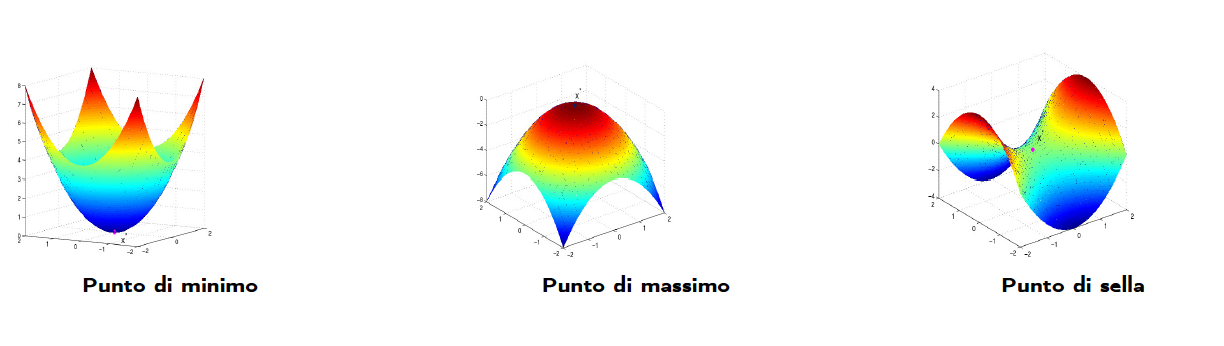
\includegraphics[width=0.9 \textwidth]{sections/images/opt1.png}


\begin{theorem} (Second order optimality condition)
    Let $f: \set{A} \in \set{R}$, with $\set{U} \subseteq \set{R}^n$ open set. If $\vec{x}^* \in \set{U}$ is a local minimum point for $f$ and $f$ is twice differentiable around $\vec{x}^*$, then
    $$ \nabla{f}(\vec{x}^*) = 0 \text{ and } \nabla^2{f}(\vec{x}^*) \text{ is positive semidefinite} $$
\end{theorem}
Note that this is a necessary condition.


\begin{theorem}
    If $f: \set{R}^n \rightarrow \set{R}$ is twice differentiable with continuity around $\vec{x}^* \in \set{R}^n$ and $\nabla{f}(\vec{x}^*) = 0$ and $\nabla^2{f}(\vec{x}^*)$ is positive definite, then $\vec{x}^*$ is a strict local minimum point.
\end{theorem}

\begin{definition}
    $\set{C} \subset \set{R}^n$ is a \textit{convex set} if $\forall\vec{x}, \vec{y} \in \set{C}$ and $\theta \in [0, 1]$ we have
    $$ \theta\vec{x} + (1 - \theta)\vec{y} \in \set{C} $$
\end{definition}

\begin{definition}
    Let $f: \set{D} \rightarrow \set{R}$, with $D \subset \set{R}^n$ convex set. Then $f$ is a \textit{convex function} if $\forall\vec{x}, \vec{y} \in \set{D}$, $\theta \in [0, 1]$ we have
    $$ f(\theta x + (1 - \theta)\vec{y}) \leq \theta f(\vec{x}) + (1 - \theta)f(\vec{y}) $$
\end{definition}

\begin{proposition}
    We have the following:
    \begin{itemize}
        \item If $f$ is twice differentiable in $\vec{x}$ and convex (resp. strictly convex), then $\nabla^2{f}(\vec{x})$ is positive semidefinite (resp. positive definite)
        \item If $f$ is a convex function then each point of local minimum is a point of global minimum
        \item If $f$ is strictly convex then there exists a unique point of global minimum
    \end{itemize}
\end{proposition}


\subsection{Iterative methods}
Iterative methods can be formulated as follows: given an initial vector $\vec{x}_0 \in \set{R}^n$, compute for $k \geq 0$ until convergence
$$ \vec{x}_{k+1} = g(\vec{x}_k) $$
where $g$ is an arbitrary function. We have that $\vec{x}_k \rightarrow \vec{x}^*$ for $k \rightarrow \infty$, where $\vec{x}^*$ is a stationary point (local minimum).

Since, for obvious reasons, we can't compute an infinite number of terms, we need to set a \textit{stopping criterion}. Some examples are:
\begin{itemize}
    \item \textit{absolute criterion} based on first order condition, $\norm{\nabla{f}(\vec{x}_k)} < \tau_A$, where $\tau_A$ is the chosen tolerance
    \item \textit{relative criterion}, $\frac{\norm{\nabla{f}(\vec{x}_k)}}{\norm{f}(\vec{x}_0)} < \tau_R$, where $\tau_R$ is the chosen tolerance
    \item \textit{absolute criterion} on succeeding values, $\norm{\vec{x}_{k+1} - \vec{x}_k} < \tau_{AP}$, where $\tau_{AP}$ is the tolerance
    \item \textit{relative criterion} on succeeding values, $\frac{\norm{\vec{x}_{k+1} - \vec{x}_k}}{\vec{x}_k} < \tau_{RP}$, where $\tau_{RP}$ is the tolerance
\end{itemize}

\textbf{Convergence speed}
In order to evaluate how fast the algorithm approximates the solution and to compare two or more different algorithms, we define the \textit{convergence speed}.

 Let $\vec P{x}_k$ be a sequence converging to $\vec{x}^*$.
\begin{itemize}
    \item \textbf{Q-linear} if it exists $r \in (0,1)$:
    $$\frac{\|\vec{x}_{k+1}-\vec{x}^*\|}{\|\vec{x}_{k}-\vec{x}^*\|} \leq r, \ \ \forall k > k^*$$
    Hence the distance from the solution decreases at each iteration of a constant factor.
    \item \textbf{Q-superlinear} if 
    $$\lim_k \frac{\|\vec{x}_{k+1}-\vec{x}^*\|}{\|\vec{x}_{k}-\vec{x}^*\|}=0$$
    \item \textbf{Q-quadratic}
    if $$\frac{\|\vec{x}_{k+1}-\vec{x}^*\|}{\|\vec{x}_{k}-\vec{x}^*\|^2} \leq M, \ \ \forall k > k^*$$
\end{itemize}

\textbf{Observation} We remark that the classical iterative optimization methods converge to a \textbf{stationary point} of the objective function. The stationary point not always is the global minimum of the function.


\subsection{Descent methods}
Descent methods are iterative methods that can be formulated as follows: given an initial vector $\vec{x}_0 \in \set{R}^n$, compute for $k \geq 0$ until convergence
$$ \vec{x}_{k+1} = \vec{x}_k + \alpha_k\vec{p}_k $$
where $\vec{p}_k$ is a suitably chosen descent direction and $\alpha_k$ is a positive parameter called \textit{stepsize} that measures the step along the direction $\vec{p}_k$. \\
This direction is called a \textit{descent direction} if   that there exists $\alpha_k > 0$ such that
$$ f(\vec{x}_k + \alpha_k\vec{p}_k) < f(\vec{x}_k) $$
We have that:
$$
    \begin{aligned}
        &\transp{\vec{p}}_k\nabla{f}(\vec{x}_k) < 0 &\text{ if } \nabla{f}(\vec{x}_k) \neq 0\\
        &\vec{p}_k = 0 &\text{ if } \nabla{f}(\vec{x}_k) = 0
    \end{aligned}
$$
provided that $f$ is continuously differentiable around $\vec{x}_k$.


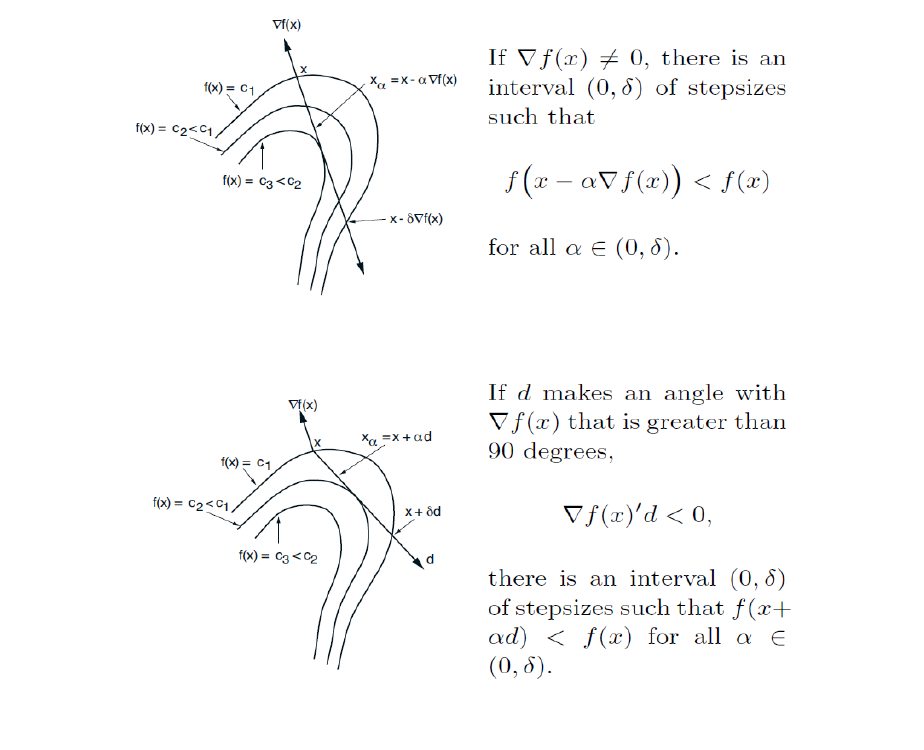
\includegraphics[width=0.9 \textwidth]{sections/images/opt3.png}

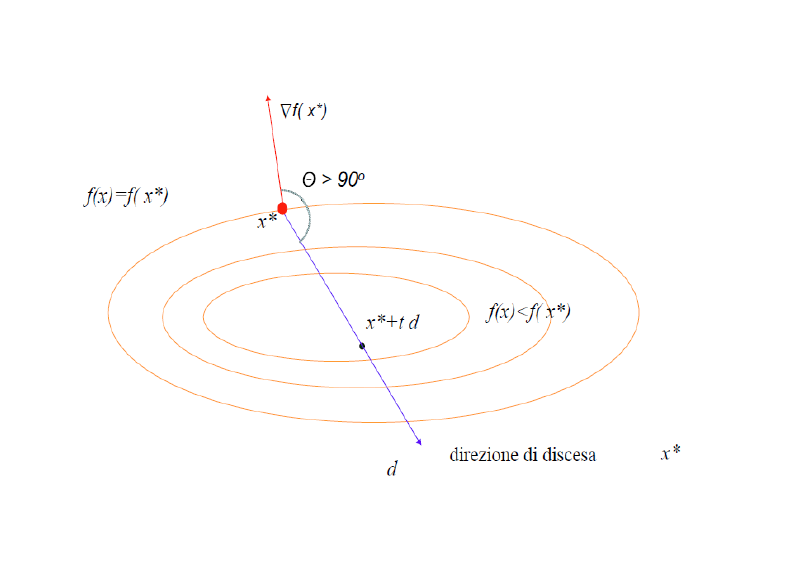
\includegraphics[width=0.7 \textwidth]{sections/images/opt4.png}

The choice of $\vec{p}_k$ corresponds to different methods.

\textbf{The choice of the step size}.

We observe that the choice of $\alpha_k$ so that:
$$f(\xx_{k+1})<f(\xx_k)$$ 
\textbf{doesn't guarantee the convergence of the method}.\\
Hence the choice of the step size is very important in a gradient descent method. If the step size is too small, the descent can be too slow. However, if the step size is too large, the method fails to converge. The step size is then usually chosen by a \textit{line search} algorithm implemented with a backtracking algorithm, where an iterative procedure decreases the value of the step size $\alpha$ until suitable conditions for the convergence of the method are satisfied. The method is called \textit{line search} since the new iterate $\xx_{k+1}$ is searched along the line $p_k$.

\begin{itemize}
    \item \textit{Exact line search}. $\alpha_k$ is chosen as the minimum of the function
    $$\Phi: R \longrightarrow R, \ \ \Phi(\alpha)=f(\xx_k+\alpha \vec{p}, \ \ \alpha \geq 0$$
    It is not the best way of choosing $\alpha_k$ in terms of converge speed of the algorithm.
    \item \textit{inexact line search}. $\alpha_k$ is chosen to belong to intervals where the algorithm convergence is guaranteed. The most common conditions which guarantees the convergence are the \textbf{Wolfe} conditions. 
    
    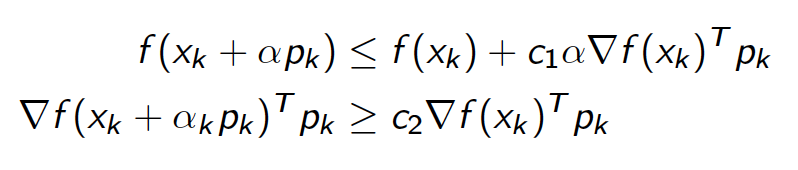
\includegraphics[width=0.7 \textwidth]{sections/images/opt5.png}
    
    with $0<c_1<c_2<1$.
    
    The first condition (Armijo condition) prevents ensures that $\alpha_k$ is not too large but it allows $\alpha_k$ to be too small. In this case the algorithm becomes very slow.\\
    The second condition (curvature condition) is a \textit{sufficient displacement} condition, preventing $\alpha_k$ from being too small.
    
    Since the curvature condition is computationally expensive, we can prove that the convergence is guaranteed if we apply a \textit{backtracking} algorithm that progressively reduces a starting values of $]\alpha$ usually set at one until the Armijo condition is satisfied. In the algorithm, a check condition ensures that $\alpha_k$ becomes not too small. In that case, the descent method is interrupted without convergence.
    
     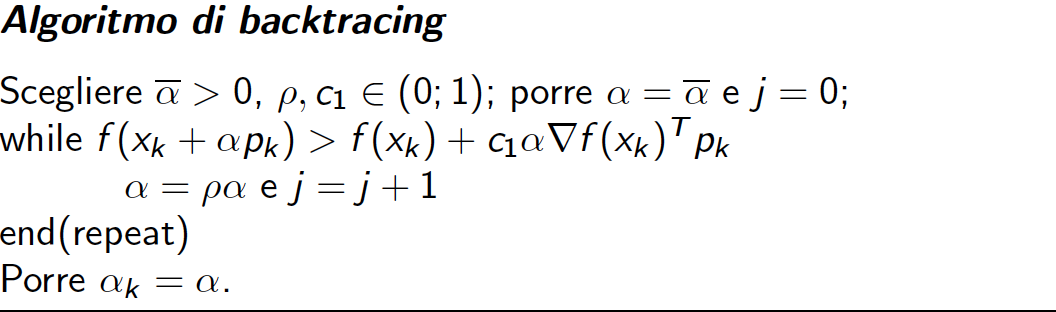
\includegraphics[width=0.7 \textwidth]{sections/images/opt6.png}
\end{itemize}



\subsubsection{Gradient descent method }

Gradient descent method is a first order optimization methods where the descent direction 
 is set as $\vec{p}_k = -\nabla{f}(\vec{x}_k)$.
 Thus
$$ \vec{x}_{k+1} = \vec{x}_k - \alpha\nabla{f}(\vec{x}_k) $$

A graphical representation can be seen in Figure \ref{fig:2}.

\begin{figure}
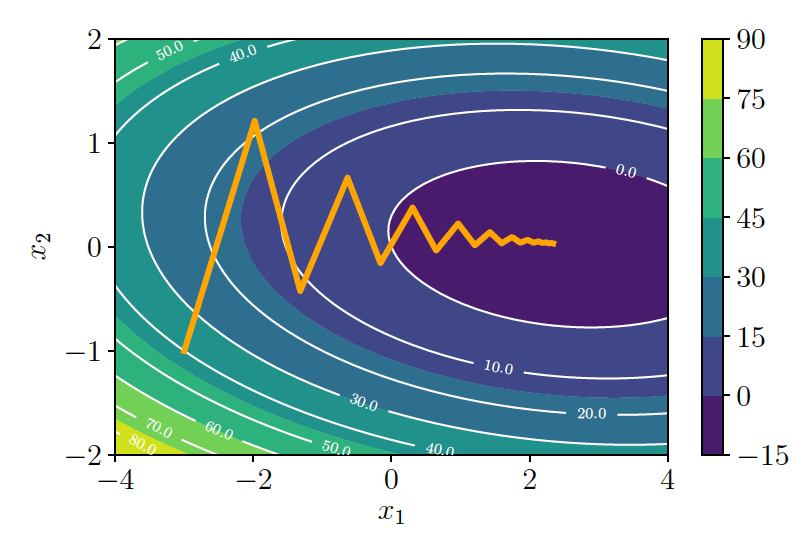
\includegraphics[width=0.7 \textwidth]{sections/images/opt2.png}
\caption{Gradient descent method on level curves of a quadratic function}
\label{fig:1}\end{figure}

The convergence speed of gradient methods is linear. In general, it can be quite slow.
 We can introduce a speeding technique called \textit{gradient descent with momentum}.
 It introduces a new term \textit{remembering} what happened in the previous iteration.
 The formula to update $\xx_k$ becomes:
 
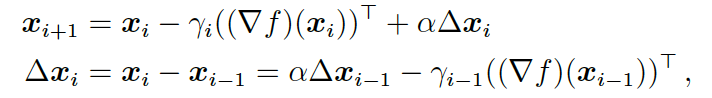
\includegraphics[width=0.7 \textwidth]{sections/images/opt7.png}

\subsubsection{Newton method}
It uses second order information of $f$, i.e. The Hessian of $f$.

The direction is set as
$$ \vec{p}_k = -\inv{H}_f(\vec{x}_k)\nabla{f}(\vec{x}_k) $$
provided that $\mat{H}_f$ is positive definite within a sufficiently large neighborhood of $\vec{x}^*$. At each iteration $\vec{p}_k$ is computed as a solution of the following linear system
$$ \mat{H}_f(\vec{x}_k)\vec{p}_k = \nabla{f}(\vec{x}_k) $$

\textbf{Convergence properties}
\begin{itemize}
    \item $\vec{p}_k$ is a decsent direction only if $\mat{H}_f$ is positive definite.
    \item The convergence properties are strictly realated to the Hessian matrix.
    \begin{proposition}
        If $f \in C^2(\Omega)$ and $\mat{H}_f$ is a Liptschiz function around $\xx^*$, i.e.
        $$|f(\xx) -f(\vec{y})| \leq K \|\xx-\vec{y} \|$$
        and $\mat{H}_f$ is positive definite then:
      if $\xx_0$ is near a stationary point $\xx^*$, then the sequence $\xx_k$ converges quadratically.
    \end{proposition}
    
\end{itemize}

\subsubsection{Possible changes in Newton methods}

\begin{itemize}
    \item 
 Approximate 
$\mat{H}_f(\vec{x}_k)$ with a positive definite matrix $\mat{B}_f(\vec{x}_k)$.
$$ \mat{H}_f(\vec{x}_k) \simeq \mat{B}(\vec{x}_k) $$ or by only using the first derivatives (\textit{Inexact Newton} methods).
\item Solve the linear system to compute the direction $p_k$ with iterative methods
\end{itemize}

\textbf{The role of the starting guess $\xx_0$.} We remark that the descent algorithms converge to a local minimum of the objective function. The value of the assigned vector $\xx_0$ starting the iterative procedure determines to which local minimum the algorithm converges. Obviously, we do not know a priori where the local (global) minima are located. If we have an estimate of the value we want to approximate, we can choose $\xx_0$ as near as possible to that value. In any case, we are not guaranteed which local minimum the algorithm converges to. In practice, we see that changing the starting guess, the result of algorithm can drastically change.

\subsection{Convex optimization}
Convex quadratic functions take the following form:
$$ q(\vec{x}) = \frac{1}{2}\transp{\vec{x}}\mat{Q}\vec{x} + \transp{\vec{c}}\vec{x}\ (+ \vec{w}) $$
with $\vec{x}, \vec{c} \in \set{R}^n$ and $\mat{Q} \in \set{R}^{n \times n}$ symmetric positive definite. A typical quadratic optimization problem is the least square problem
$$ \min{\norm{\mat{A}\vec{x} - \vec{b}}^2} $$
The objective is to minimize
$$
    \begin{aligned}
        \frac{1}{2}\norm{\mat{A}\vec{x} - \vec{b}}^2 &= \frac{1}{2}\transp{(\mat{A}\vec{x} - \vec{b})}(\mat{A}\vec{x} - \vec{b}) =\\
        &= \frac{1}{2}(\transp{\vec{x}}\transp{\mat{A}} - \transp{\vec{b}})(\mat{A}\vec{x} - \vec{b}) =\\
        &= \frac{1}{2}(\transp{\vec{x}}\transp{\mat{A}}\mat{A}\vec{x} - \transp{\vec{x}}\transp{\mat{A}}\vec{b} - \transp{\vec{b}}\mat{A}\vec{x} + \transp{\vec{b}}\vec{b}) =\\
        &= \frac{1}{2}\transp{\vec{x}}\transp{\mat{A}}\mat{A}\vec{x} - \transp{\vec{b}}\mat{A}\vec{x} + \frac{1}{2}\transp{\vec{b}}\vec{b}
    \end{aligned}
$$
which can be rewritten in quadratic form by setting $\mat{Q} = \transp{\mat{A}}\mat{A}$ and $\transp{\vec{c}} = -\transp{\vec{b}}\mat{A}$
We have
$$ \nabla{f}(\vec{x}) = \transp{\mat{A}}\mat{A}\vec{x} - \transp{\mat{A}}\vec{b}$$
and setting $\nabla{f}(\vec{x}) = 0$ we obtain the normal equations
$$ (\transp{\mat{A}}\mat{A})\vec{x} = \transp{\mat{A}}\vec{b} $$

A strictly convex function frequently encountered in applications is the quadratic function:
$$f(\xx)=\frac{1}{2} \xx^T Q \xx + \vec{b} ^T \xx$$
where $Q$ is a square matrix of size $n \times n$ symmetric and positive definite, $\vec{b} \in \mathbf{R}^n$.

In this particular case we have:
$$\nabla f(\xx)=Q \xx- \vec{b} \ \ \nabla^2 f(\xx)=A$$
Hence the unique minimizer of $f$ is the solution of the linear system representing the first order conditions $\nabla f(\xx)=0$:
$$Q \xx= \vec{b}$$

\textbf{Steepest descent method.} The \textit{steepest descent method} is the gradient method applied to a quadratic convex function with exact line search.

\begin{figure}
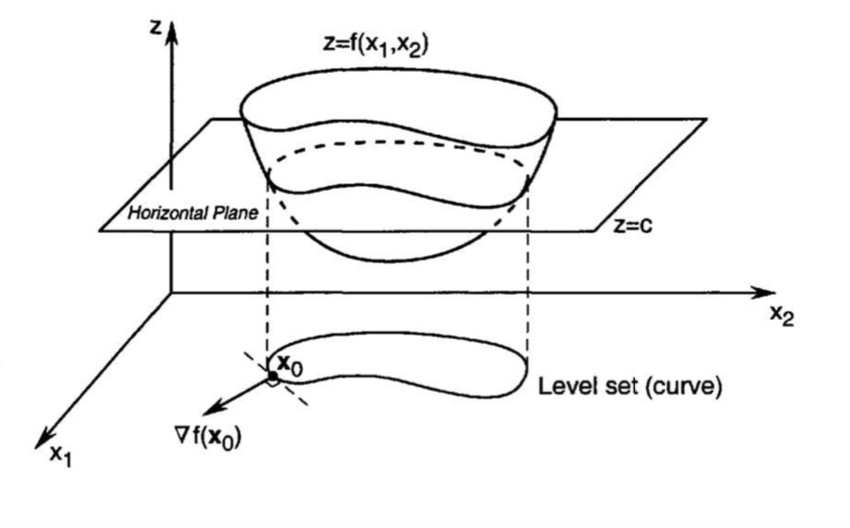
\includegraphics[width=0.7 \textwidth]{sections/images/opt8.png}
\caption{Descent direction in a gradient method}
\label{fig:2}\end{figure}

The step length $\alpha_k$ is computed as the global minimum of the univariate function of the variable $\alpha$ (in this case the function is convex):

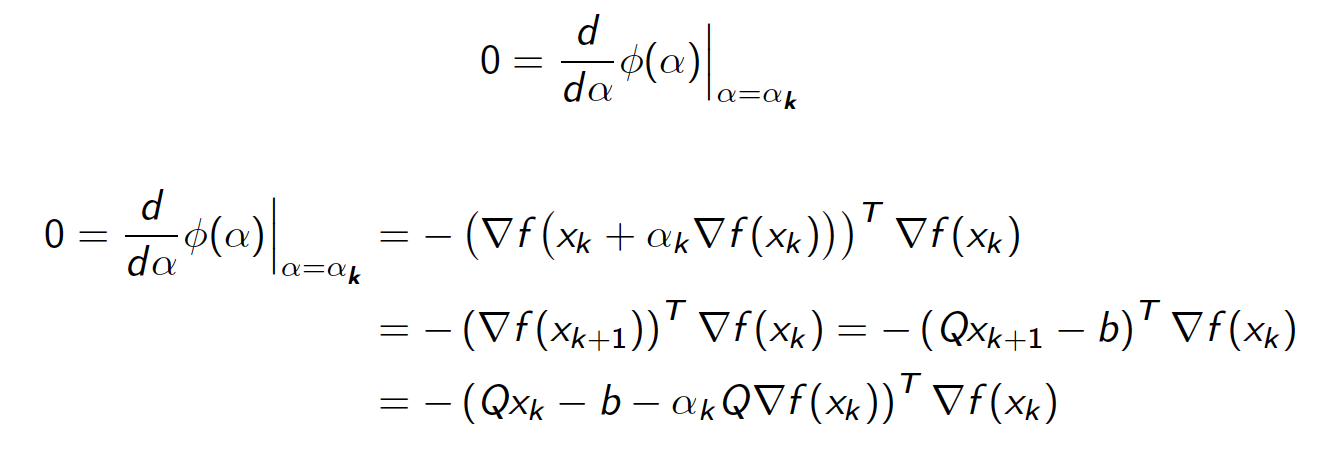
\includegraphics[width=0.9 \textwidth]{sections/images/opt12.png}

Hence:

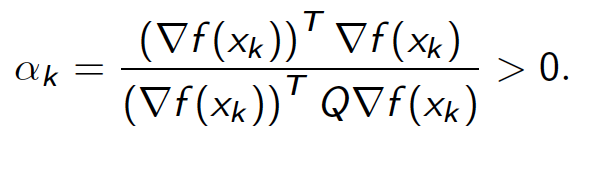
\includegraphics[width=0.5 \textwidth]{sections/images/opt13.png}

 The final algorithm can be written as:
 
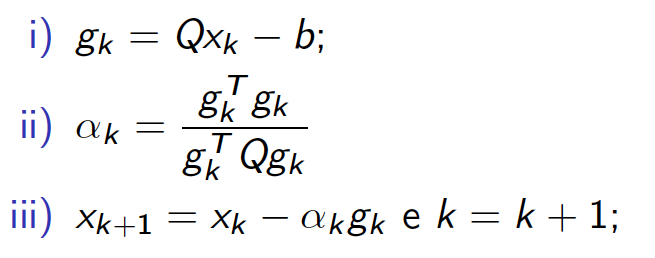
\includegraphics[width=0.6 \textwidth]{sections/images/opt14.png}


The gradient can be modified by considering Q-conjugate directions $\vec{p}_i$:
$$\vec{p}_i^T Q \vec{p}_j=0, \ \ if i \neq j$$

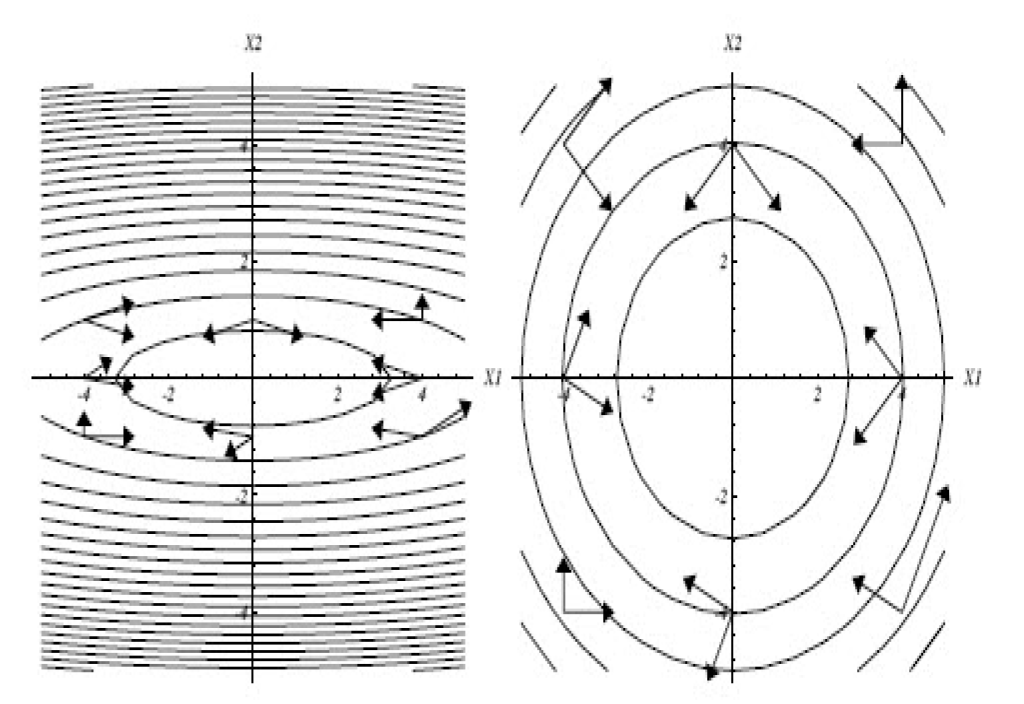
\includegraphics[width=0.6 \textwidth]{sections/images/opt9.png}
   
The \textit{Conjugate Gradient } (CG) algorithm is a very fast iterative algorithm for the minimization of a quadratic function (i.e. an iterative method for the solution of a linear system $Q\xx=\bb$ with $Q$ symmetric and positive definite).
It can be described by the following instructions:

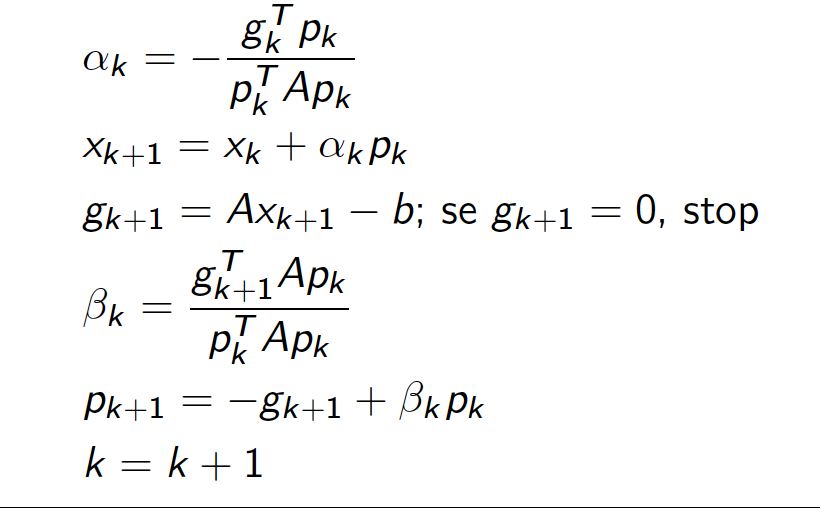
\includegraphics[width=0.6 \textwidth]{sections/images/opt10.png}

\begin{proposition}
If $A$ is symmetric and positive definite and it has at most $s$ distinct eigenvalues, then the CG method converges, in exact arithmetic, in at most $s$ iterations.
\end{proposition}

For any symmetric and positive definite matrix $Q$, we define the \textit{energy norm}:
$$\| \xx \|_Q=\sqrt{\xx^T Q \xx}$$ 
Concerning the convergence speed of Gradient Descent and Conjugate Gradient algorithms when applied to a quadratic function, we have the following results:
\begin{itemize}
\item For the steepest descent method it holds:
    $$ \| \xx_k - \xx^* \|_Q^2 \leq \left(\frac{K(Q)-1}{K(Q)+1}\right)^2 \| \xx_{k-1} - \xx^*\|_Q^2$$
    \item For the CG method it holds:
    $$ \| \xx_k - \xx^* \|_Q^2 \leq \left(\frac{K(Q)-1}{K(Q)+1}\right) \| \xx_{k-1} - \xx^*\|_Q^2 $$
\end{itemize}
where $k$ is the iteration number and $K(Q)$ is the condition number of $Q$.
Hence the CG method is quite faster then the Gradient descent method.

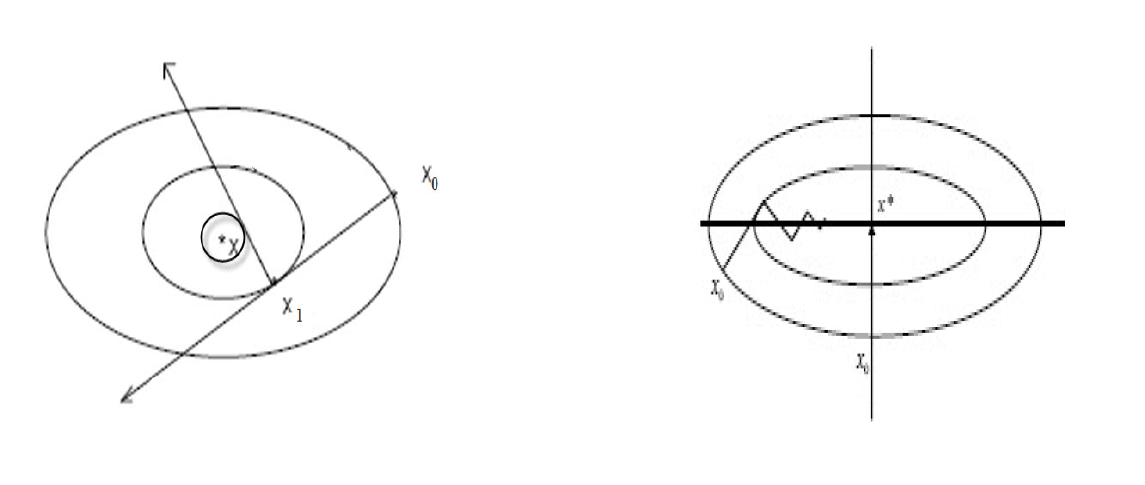
\includegraphics[width=0.6 \textwidth]{sections/images/opt15.png}

\subsection{Stochastic optimization}
The objective function in some ML problems is related to probabilistic events and it can take the following form
$$ G(\vec{x}) = \sum_{i = 1}^{n}{G_i(\vec{x})} $$
with $G: \set{R}^n \rightarrow \set{R}$. Each $G_i$ is the so called \textit{loss function} associated with the $i$-th observation in the dataset.
For example in a supervised classification problem we minimize the \textit{empirical risk function} $R_n:\mathbf{R}^d \longrightarrow \mathbf{R}$ defined as the sum of loss functions $l, \ i=1, \ldots n$ for all the examples $x_i$:
$$R_n(\vec{w})=\frac{1}{n} \sum_{i=1}^n l(h_(x_i,\vec{w}))$$
where the loss function $l$ is related to the probability distribution of the examples $x_i$.


In the case of standard (or \textit{batch}) gradient descent, the iteration is
$$
    \begin{aligned}
        \vec{x}_{k+1} &= \vec{x}_k - \alpha_k\nabla{G}(\vec{x}_k)\\
        &= \vec{x}_k - \alpha_k\sum_{i=1}^{n}{\nabla{G_i}(\vec{x}_k)}
    \end{aligned}
$$
When there are millions of examples, it is very expensive to compute the gradient $\nabla G(\xx)$.

In \textit{stochastic gradient descent} the true gradient $\nabla{G}(\vec{x}_k)$ is approximated at each iteration by the gradient at a single observation $\nabla{G_i}(\vec{x}_k)$, with $i = 1, \hdots, n$ randomly picked. The iteration step becomes
$$ \vec{x}_{k+1} = \vec{x}_k - \alpha_k\nabla{G_i}(\vec{x}_k) $$

A compromise between batch gradient descent and stochastic gradient descent is to compute the gradient against a set (called \textit{mini-batch}) of randomly picked observations. This method is therefore called \textit{mini-batch stochastic gradient descent}. The iteration step becomes
$$ \vec{x}_{k+1} = \vec{x}_k - \alpha_k\sum_{i \in M}{\nabla{G_i}(\vec{x}_k)},\ \ \ M \subset \{1, \hdots, n\} $$
The selection of the set $M$ can be performed in different random ways and it can also depend on the iterate $\xx_k$.

The step size $\alpha_k$ can be fixed or dynamically computed with a line search procedure. Both the choices are interesting in ML.

Each iteration is now very cheap and $\xx_1, \ldots \xx_k $ is a stochastic process, whose behaviour is determined by the random sequence $i_1, \ldots i_k$ of the indices of the computed component of the gradient at each iteration (in the case of a single component or depending on the random sequence of the mini-batches).
Even if the direction $-\nabla G_{i_k}(\xx_k)$ might NOT be a descent direction from $\xx_k$, but it is a descent direction \textit{in expectation}. This is proved to converge \textit{in expectation} to a local minumum of $G$.

Stochastic gradient descent is less computationally demanding with respect to batch gradient descent, but its convergence speed is lower. The convergence of stochastic gradient descent has been analyzed using the theories behind convex minimization and stochastic approximation.
Since in ML we do not need a very precise localization of the minimum of the function, stochastic (or mini-batch) gradient represents a very good compromise between precision and computational cost and it is widely used in practice, such as in neural network training algorithms.

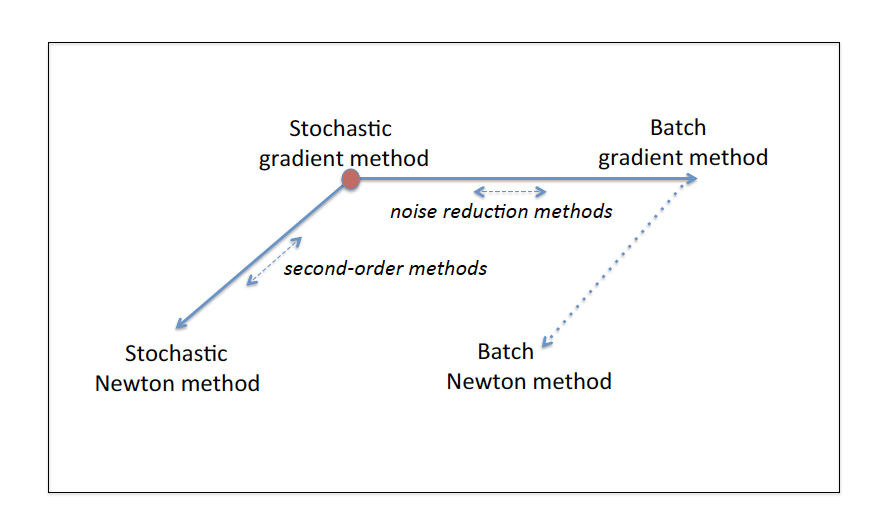
\includegraphics[width=0.6 \textwidth]{sections/images/opt11.png}

In a similar way, other optimization algorithms, such as Newton-like methods , can be implemented with a stochastic (or mini-batch) gradient computation.
More details can be found in \textit{Optimization for large scale machine learning, Siam Review, vol. 60, n.2, pag. 223-311, 2018}, where some convergence results are presented in the case of strictly convex functions.

\subsection{Non-linear least squares problem}
In non-linear least squares problems we have residuals defined as $\vec{r}: \set{R}^n \rightarrow \set{R}^m$, where $n$ is the dimension of the space of the data and $m$ is the dimension of the space of the unknowns. Each $r_i(\vec{x})$ is a non-linear function and the minimization of the residuals can be written as
$$ \min{\norm{\vec{r}(\vec{x})}^2} = \min{\sum_{i = 1}^{m}{r_i^2(\vec{x})}} $$
We can write the gradient of $f: \set{R}^m \rightarrow \set{R}$, $f = \frac{1}{2}\sum_{i = 1}^{m}{r_i^2(\vec{x})}$ as
$$ \nabla{f}(\vec{x}) = \sum_{i = 1}^{m}{r_i(\vec{x})\nabla{r_i}(\vec{x})} = \transp{\mat{J}}_r(\vec{x}) \cdot \vec{r}(\vec{x}) $$
and the hessian of $f$ as
$$
    \begin{aligned}
        \mat{H}_f(\vec{x}) &= \sum_{i = 1}^{m}{\left(\nabla{r_i}(\vec{x}) \cdot \nabla^T{r_i}(\vec{x}) +\nabla{r_i}(\vec{x}) \cdot \transp{\mat{H}}_{r_i}(\vec{x})\right)} =\\
        &= \transp{\mat{J}}_r(\vec{x}) \cdot \mat{J}_r(\vec{x}) + \sum_{i = 1}^{m}{\nabla{r_i}(\vec{x}) \cdot \transp{\mat{H}}_{r_i}(\vec{x})}
    \end{aligned}
$$

These formulas can be very expensive to compute. The methods used to solve these problems are:
\begin{itemize}
    \item \textit{gradient methods}
    \item \textit{Newton-like methods}
    \item \textit{Gauss-Newton method}, where $\vec{p}_k$ is computed as
    $$ (\transp{\mat{J}}_r \cdot \mat{J}_r)(\vec{x}_k) \cdot \vec{p}_k = -\transp{\mat{J}}_r(\vec{x}_k) \cdot \vec{r}(\vec{x}_k) $$
    \item \textit{Levenberg-Marquardt method}, adds regularization because $(\transp{\mat{J}}_r \cdot \mat{J}_r)$ can be ill-conditioned. $\vec{p}_k$ is computed as
    $$ (\transp{\mat{J}}_r(\vec{x}_k) \cdot \mat{J}_r(\vec{x}_k) + \lambda\mat{I}) \cdot \vec{p}_k = -\transp{\mat{J}}_r(\vec{x}_k) \cdot \vec{r}(\vec{x}_k) $$
\end{itemize}

\subsection{Constrained optimization. Lagrange multipliers}

We consider now the problem
\begin{eqnarray}
& min_x G(\xx) \\
& s.t. \ h_i(\xx) \leq 0 \ i=1, \ldots m
\label{eq:1}
\end{eqnarray}

A possible way of solving \eqref{eq:1} is to introduce the \textit{Lagrange multipliers} $\lambda_i \geq 0, \ i=1, \ldots m.$ The \textit{Lagrangian} function associated to problem \eqref{eq:1}. is:
$$L(\xx, \vec{\lambda})=G(\xx)+\sum_{i=1}^m \lambda_i h_i(\xx)$$

Many numerical methods use also the concept of duality. The minimization in a set of variables, say $\xx$ is moved in the minimization in another set of variables, say $\vec{\lambda}$. Given a minimization problem, there is not a unique way of getting duality. We consider now the so called \textit{Lagrangian duality}.

\begin{definition}
To the \textit{primal problem} \eqref{eq:1} with primal variables $\xx$, we associate the \textit{Lagrangian dual problem} in the form:
\begin{eqnarray*}
max_{\vec{\lambda}\in R^m} D(\vec{\lambda}) \\
s.t. \ \vec{\lambda} \geq 0
\end{eqnarray*}
where $D(\vec{\lambda})=min_{\xx \in R^n} L(\xx, \vec{\lambda})$ and $\vec{\lambda}$ are the \textit{dual variables}.
\end{definition}

The first one is the \textit{minimax problem}. If the solution of $min_{\xx \in R^n} L(\xx, \vec{\lambda})$ can be easily performed, then all the problem can be effortlessly computed. In fact, the maximization problem of $D(\vec{\lambda})$ is a concave problem, whose maximum is quite simple to find, even if $G$ and $h_i$ are not convex.

A particular case is the case when the functions $G$ and $h_i$ are linear. In this case we obtain the \textit{linear programming problem}

% \subsection{Regularization}
% \textit{Regularization} techniques can be used to slightly change ill-conditioned matrices. The simplest method is to add a diagonal matrix multiplied by a \textit{regularization parameter}, $\lambda\mat{I}$. Regularization also attempts to impose Occam's razor on the solution, meaning that it helps generate a simpler solution which is less affected by noise. For example, in Bayesian statistics we can impose certain prior distributions (regularization term) on model parameters
% $$ \hat{\theta}_{MAP} = -\argmin_{\theta}{\sum_{i = 1}^{n}{\log{f_X(x_i \mid \theta)}}} + \lambda\log{p(\theta)} $$


 

%  \section{Probability and Statistics}
%  The objective of probability is to quantify the uncertainty: in the data, in the results, in the ML model...
Hence we introduce the concepts of random variable and probability distribution.
In ML probability is often used to formalize the design of automated reasoning systems.
Moreover, in ML we are interested in generalizing the errors produced by our algorithm. Really, we do not know how the algorithm will perform on new data. This analysis involves both probability, which captures the uncertainty by random variables, and statistics, which uses probability to infer on the unknown behaviour of events.

In ML there are two main interpretations of probability: the \textit{Bayesian} interpretation and the \textit{frequentist} interpretation.

Dear The Bayesian interpretation is also called \textit{subjective probability} because it is used to quantify the degree of uncertainty that the user has about an event (Bishop, Pattern Recognition and Machine Learning, 2006).\\
The frequentist interpretation considers the frequency of events of interest with respect to the total number of events occurred.

\subsection{Basics of probability}

\begin{definition}
    A \textit{random experiment} is an experiment whose outcome is determined by chance (e.g. roll of a die).
\end{definition}

\begin{definition}
    The \textit{sample space} is the set of all possible results of a random experiment.
\end{definition}

Examples. Toss of a coin, roll of a die, drawing a card form a deck  or extraction of ball from an urn.

\begin{definition}
    An \textit{event} is a collection of results. It is also defined as a subset of the sample space.
\end{definition}

Examples of events.

\begin{definition}
    The \textit{space of the events} $S(A)$ is the set of all the possible events.
\end{definition}

\begin{definition}
    The \textit{probability of an event $A$} is a function $P: S(A) \rightarrow [0,1] \in \set{R}$ that associates each event $A$ to a number called probability of $A$.
\end{definition}

\begin{proposition}
    Each probability function $P$ satisfies:
    
    \begin{itemize}
        \item $P(A) \geq 0$
        \item $P(S) = 1$
        \item if $A_1, A_2, \hdots, A_n$ are disjoint events ($A_1 \cap A_2 \cap \hdots \cap A_n = \emptyset$) then
        $$ P(A_1 \cup A_2 \cup \hdots \cup A_n) = \sum_{i=1}^{n}{P(A_i)} $$
    \end{itemize}
\end{proposition}

\begin{definition}
    The \textit{conditional probability} of an event $B$ given the event $A$ is defined as
    $$ P(B \mid A) = \frac{P(A \cup B)}{P(A)} $$
\end{definition}

Example. Suppose to toss a coin three times. Consider the events:
$A\{ two crosses C occur\}$, $B=\{one head H and one cross C occur \}$. Compute $P(A|B)$ and $P(B|A)$.

\begin{proposition}
    For any fixed $A$, with $P(A) > 0$:
    
    \begin{itemize}
        \item $P(B \mid A) \geq 0, \forall B \subset S$
        \item $P(S \mid A) = 1$
        \item $B_1, B2, \hdots, B_n$ disjoint events
        $$ P\left(\bigcup_{i = 1}^{n}{B_i} \mid A\right) = \sum_{i=1}^{n}P(B_i \mid A) $$
        \item $\forall A_1, A_2, \hdots, A_n$ events:
        $$ P(A_1 \cap \hdots \cap A_n) = P(A) \cdot P(A_2 \mid A_1) \cdot \hdots \cdot P(A_n \mid A_1 \cap \hdots \cap A_{n-1}) $$
    \end{itemize}
\end{proposition}

\begin{definition}
    Two events $A$ and $B$ are \textit{independent} iff
    $$ P(A \cap B) = P(A) \cdot P(B) $$
    Two events which are not independent are called \textit{dependent}.
\end{definition}

\begin{theorem}
    Given $A, B$ disjoint events, $A \cup B = S$, we have that
    $$ P(B \mid A) = \frac{P(A \mid B)P(B)}{P(A)} $$
    The theorem can be extended to multiple events $B_1, \hdots, B_n$ pairwise disjoint ($B_i \cap B_j = \emptyset,\ \forall i \neq j$) and exhaustive ($B_1 \cup \hdots \cup B_n = S$)
    $$ P(B_i \mid A) = \frac{P(A \mid B_i)P(B_i)}{\sum_{i=j}^{n}{P(A \mid B_j)P(B_j)}} $$
\end{theorem}

\subsection{Random variables}
The \textit{random variables} associates events to numbers. In this way we can mathematically describes the probability
of events occurring.
\begin{definition}
    A \textit{random variable} is a function $X: S \rightarrow \set{R}$ that associates each outcome $w \in S$ to a number $x \in \set{R}$
    $$ X(w) = x $$
\end{definition}

\begin{definition}
    The set of all the possible values of a random variable $X$ is called \textit{target space or support of $X$}, $S_X$.
\end{definition}

Examples. 
\begin{enumerate}
\item Toss a coin twice. The sample space is $S=\{HH, CH, HC, CC\}$. Consider the random variable $X=\{number of C\}$. Determine the values of X and its target space.
\item  Repeat the Roll of a die  until you get 6. Consider the random variable $Y=\{ number of rolls \}$.
Determine the values of Y and its target space.
\item Monitor the arrival of a client in a bank. Consider $Z=\{ Time before the arrival of the client \}$.Determine the values of Z and its target space.

\end{enumerate}

If the target space (support) (case of X and Y) is a countable set then the random variable is called \textit{discrete}.

If the target space (support) (case of Z) is a non countable set then the random variable is called \textit{continuous}.

Associated to the random variables we have  probability functions which describe how the probability of events id distributed. We call \textit{univariate} distribution when we consider the distribution of  a single random variable and \textit{multivariate} distribution when we have more than one random variable.

\subsubsection{Discrete random variables and probability mass function}

Each discrete random variable has a function associated to itself, called \textit{probability mass function} (PMF) which describes the probability mapping between the event and the probability of outcome of the random variable.

$$ p_X: S_X \rightarrow [0,1] \in \set{R} $$
such that
$$ p_X(x) = P(X = x),\ x \in S_X $$
and
$$ \sum_{x \in S_X}{f_X(x)} = 1 $$

\begin{definition}
    The \textit{expectation} of a discrete random variable is defined as
    $$ \mu = \mathbb{E}[X] = \sum_{x \in S_X}{xf_X(x)} $$
\end{definition}

The expectation of a function $g(X)$ is defined as
$$ \mathbb{E}[g(X)] = \sum_{x \in S_X}{g(x)p_X(x)} $$

\begin{definition}
    The \textit{variance} of a discrete random variable is defined as
    $$ \sigma^2 = \mathbb{E}[(X - \mu)^2] = \sum_{x \in S_X}{(x - \mu)^2p_X(x)} = \mathbb{E}[X^2] - \mathbb{E}^2[X] $$
\end{definition}

Some examples of probability mass function are:

\begin{itemize}
    \item the \textit{discrete uniform distribution} (n is the dimension of the support)
    $$ p_X(x) = \frac{1}{n} $$
    \item the \textit{Poisson distribution}
    $$ p_X(x) = e^{-\lambda}\frac{\lambda^x}{x!} $$
    which has $\mu = \lambda$ and $\sigma^2 = \lambda$
\end{itemize}

\textbf{Multivariate discrete distributions}

While in the univariate case, the target space of a RV (random variable) is associated with a vector, in the multivariate case it is defined as the cartesian product of the single target spaces, hence fills a multidimensional array.
For example, in the case of bivariate RV, the target space $S_{XY}=S_X \times S_Y$, hence it fills a matrix.

\begin{definition}
    The \textit{joint probability mass function} of $X$ and $Y$ is defined as
    $$ p_{XY} = P(X = x_i, Y = y_j)=\frac{a_{ij}}{N},\ (x, y) \in S_{XY} $$
    where $a_{ij}$ is the element of the matrix storing all he possible values of X and Y, N is the total number of matrix elements (events). 
\end{definition}

We also write $f_{XY}$ as $p(x,y)$.
\begin{definition}
    Given $p_{XY}$ joint probability mass function of $X$ and $Y$ we define the \textit{marginal probability distribution} of $X$ as
    $$ p_X(x) = \sum_{y \in S_Y}{P(X = x, Y = y)} $$
    and the \textit{marginal probability distribution} of $Y$ as
    $$ p_Y(y) = \sum_{x \in S_X}{P(X = x, Y = y)} $$
\end{definition}

We observe that the marginal probability consider only one  RV at a time.

Example 6.2 MML

\subsubsection{Continuous random variables}

Each continuous  random variable has a function associated to itself, called \textit{probability density function} (PDF) $p(x)$ satisfying:
$$ P(a \leq X \leq b) = \int_{a}^{b}{p_X(x)dx},\ \forall[a, b] \in S_X $$
and 
$$\int_a^b p(x)dx=1$$

%\begin{definition}
%    The \textit{expectation} of a continuous random variable is defined as
%    $$ \mu = \mathbb{E}[X] = \int_{x \in S_X}{x p_X(x)} $$
%\end{definition}

%The expectation of a function $g(X)$ is defined as
%$$ \mathbb{E}[g(X)] = \int_{x \in S_X}{g(x)p_X(x)} $$

%\begin{definition}
%    The \textit{variance} of a continuous random variable is defined as
 %   $$ \sigma^2 = \mathbb{E}[(X - \mu)^2] = \int_{x \in S_X}{(x - \mu)^2f_X(x)} = \mathbb{E}[X^2] - \mathbb{E}^2[X] $$
%\end{definition}

Some examples of probability density  functions (PDF) are:

\begin{itemize}
    \item the \textit{normal distribution} (or \textit{Gaussian distribution})
    $$ p_X(x) = \frac{1}{\sigma\sqrt{2\pi}}\exp{\left(-\frac{(x-\mu)^2}{2\sigma^2}\right)} $$
    with expectation $\mu$ and standard deviation $\sigma$. The \textit{standard normal distribution} is defined with parameters $\mu = 0$ and $\sigma = 1$.
    \item the \textit{exponential distribution}
    $$ p_X(x) = \lambda e^{-\lambda x} $$
    which has mean $\mu = \frac{1}{\lambda}$ and standard deviation $\sigma = \frac{1}{\lambda}$
\end{itemize}


\subsection{Bayes' theorem}

\begin{definition}
   Given X and Y rv, let  consider the instances $X=x$. We define \textit{conditional probability of y given x} and we write $p(y|x)$ the fraction of instances for which $Y=y$.
\end{definition}

\textbf{SUM rule.}

WE show the sum rule for  discrete rv. In the case of continuous rv the sum is substituted by the  integral.

\begin{proposition}
Let $x$ and $y$ be discrete rv. Then:
$$p(x)= \sum_{y \in Y} p(x,y)$$
\end{proposition}

It is called also \textit{marginalization property} since it involves marginal distribution and joint distribution. The marginal distribution of one rv is the sum on the events on the other rv. If we have more than two rv, we can apply the sum rule to all the subsets of the random variable. For example if we have a set $x=(x_1, \ldots x_n)$ of rv, 
$$p(x_i)=\sum_{y \in (x1, \ldots x_{i-1}, x{i+1}, \ldots x_n)} p(x_1, \ldots x_n)$$

\textbf{Product rule}

\begin{proposition}
Let $x$ and $y$ be discrete rv. Then:
$$p(x,y) =p(y|x)p(x)$$
\end{proposition}

It relates the joint distribution and the conditional distribution by showing that a joint distribution can be written as the product of a marginal distribution by a conditional distribution.
Obviuosly we can interchange $x$ and $y$.

We finally state the Bayes' Theorem.

Suppose we have prior on an unobserved variable $\xx$ and we have a relationship between $x$ and another rv $y$, which is observed.
\begin{proposition}
    Let $x$ and $y$ be discrete rv.
    Then:
    $$p(x|y)=\frac{p(y|x)p(x)}{p(y)}$$
    where $p(x|y)$ is called \textit{posterior}, $p(y|x)$ is the \textit{likelihood}, $p(x)$ is the \textit{prior} and $p(y)$ is the \textit{evidence}.
    \end{proposition}
    \begin{proof}
    For the product rule we have:
$$p(x,y) =p(x|y)p(y)$$
and
$$p(x,y) =p(x|y)p(y)$$
Hence:
$$p(x,y) =p(y|x)p(x)=p(x|y)p(y)$$
From which we can derive the thesis.
\end{proof}
What's the meaning of the terms involved in the Bayes' theorem?

\begin{itemize}
    \item The \textbf{prior} represents knowledge about the discrete probability distribution of $x$, which is the latent variable we want to discern about. The choice of the prior depends on the information we can know about $x$ a priori.
    \item The \textbf{likelihood} is the probability of the observed rv $y$ given $x$. It is a distribution in $y$. We usually call it \textit{the probability of y given x}.
    \item The \textbf{posterior} is what we want to know in the Bayesian statistic. It represents what we know of $x$ having observed $y$.
    \item The \textbf{evidence} is the known probability of the observed  $y$.
\end{itemize}

As we said, we are interested in the posterior. But often is very difficult to know exactly the posterior, hence we consider only some statistic of the posterior, such as its mean or maximum. This causes loss of information. Some ML algorithms aim at finding the posterior distribution.

% \subsection{Statistics}

% We call \textit{statistic} an   index related to a rv we can measure from a sample of the rv. Examples are the mean, the variance, the standard deviation, the correlation ...

% We first introduce the \textit{expected value} of a function $g(x)$ of a univariate discrete rv X with probability density function $p(x)$ as:
%   $$\mathbb{E}[g(x)]=\sum_{x \in S_X} g(x)p(x)dx$$
%   where $S_X$ is the target space of the rv X.
  
%   If we consider a multivariate random variables $X=(X_1, \ldots X_n)$ the expected value is a vector containing as elements the expected values with respect to the single rv $X_i, i=1, \ldots n$.
  
%   \begin{definition} 
%   The \textit{mean} of a univariate rv X with states $(x_1, \ldots x_m)$ is an average defined as:
%   $$=\sum_{x_i \in S_X}x_i p(x_d=x_i)$$
%   \end{definition}
  
%   Let $\mu_X=\mathbb{E}[X](\xx)$ and $\mu_Y=\mathbb{E}[Y](\yy)$.
% \begin{definition}
%     We define the \textit{covariance} between two random variables $X$ and $Y$ as
%     $$ \text{Cov}_{XY}[x, y] = \mathbb{E}[(x - \mu_X)(y - \mu_Y)] = \mathbb{E}[XY] - \mathbb{E}[X]\mathbb{E}[Y] $$
% \end{definition}

% We have $\text{Cov}_{XX}(x, y) = \mathbb{E}[xy]-\mathbb{E}[x]\mathbb{E}[y]$

% %%%%%%%%%%%%%%%%%%%%%%%%%%%%%%%%%%%%%%%%%%%%%%%%%%%%%%%%%%%%%%%%%%%%%%%%%%%%%%%%%%%%%%%%%%%%%%%

% \begin{definition}
%     We define the \textit{correlation} between two random variables $X$ and $Y$ as
%     $$ \text{Corr}_{XY}(X, Y) = \frac{\text{Cov}_{XY}(X, Y)}{\sigma_X\sigma_Y} $$
% \end{definition}

% If $X \in \set{R}^m,\ X = (X_1, X_2, \hdots, X_m)$ and $Y \in \set{R}^n,\ Y = (Y_1, Y_2, \hdots, Y_n)$ we have that $\text{Cov}(X, Y)$ and $\text{Corr}(X, Y)$ are matrices of size $m \times n$ such that
% $$ (\text{Cov}(X, Y))_{ij} = \text{Cov}(X_i, Y_j) $$
% $$ (\text{Corr}(X, Y))_{ij} = \text{Corr}(X_i, Y_j) $$

% If $X \in \set{R}^n,\ X = (X_1, X_2, \hdots, X_n)$ we have that $\text{Cov}(X, X)$ is a symmetric positive definite matrix of size $n \times n$ whose diagonal terms are $\sigma^2_{X_i}$

% \begin{proposition}
%     If $X$ and $Y$ are two independent random variables then
%     $$ \text{Cov}(X, Y) = 0,\ \text{Corr}(X, Y) = 0 $$
% \end{proposition}

% \subsection{Inferential statistics}
% Inferential statistics tries to deduce underlying properties of the distribution of a population from which a sample is observed. The set of assumptions is called \textit{statistical model} and the assumed probability distribution is usually parametrized. These parameters are then estimated to fit the observed data as well as possible.

% We will study two methods to estimate the parameters of the assumed probability distribution:

% \begin{itemize}
%     \item \textit{maximum likelihood estimation} (MLE)
%     \item \textit{maximum a posteriori estimation} (MAP)
% \end{itemize}

% \subsubsection{Maximum likelihood estimation}
% The goal of maximum likelihood estimation is to maximize the likelihood of the observed data with respect to the parameters
% $$ L(\theta \mid x) = f_{X}(x \mid \theta) $$
% Here $f_{X}(x \mid \theta)$ is viewed as a function of the parameter $\theta$ with $x$ fixed. This should not be seen as the probability that the parameters $\theta$ are the right ones, given the observed data.

% Thus, the method of maximum likelihood estimation estimates $\theta$ as
% $$ \hat\lambda_{MLE}(x) = \argmax_{\lambda}\{{L(\theta \mid x)}\} = \argmin_{\lambda}\{{-\ln{L(\theta \mid x)}}\} $$

% \begin{example}
    Suppose $X_1, \hdots, X_n \sim \exp(\lambda)$ i.i.d. random variables with observations $(x_1, \hdots, x_n)$. We have
    $$ L(\lambda \mid x_1, \hdots, x_n) = \prod_{i=1}^{n}{\lambda e^{-\lambda x_i}} = \lambda^n e^{-\lambda\sum_{i=1}^{n}{x_i}} $$
    To find $\lambda$ we need to compute
    $$ \argmax_{\lambda}\{ \lambda^n e^{-\lambda\sum_{i=1}^{n}{x_i}} \} = \argmin_{\lambda}\{ -n\ln{\lambda} + \lambda\sum_{i=1}^{n}{x_i} \} $$
    Let's compute the derivative of $L_1(\lambda) = -n\ln{\lambda} + \lambda\sum_{i=1}^{n}{x_i}$ with respect to $\lambda$
    $$ \frac{dL_1}{d\lambda}(\lambda) = -\frac{n}{\lambda} + \sum_{i=1}^{n}{x_i} $$
    Thus, the value of $\lambda$ which minimizes $L_1$ is $\lambda = \frac{n}{\sum_{i=1}^{n}{x_i}}$.
\end{example}

% \subsubsection{Maximum a posteriori estimation}

% Assume that we want to estimate an unobserved parameter $\theta$ on the basis of observations $x$. Let $f$ be the sampling distribution of $x$, so that $f_{X}(x \mid \theta)$ is the probability of $x$ when the underlying population parameter is $\theta$. Then the function
% $$ \mathcal{L}(\theta \mid x) = f_{X}(x \mid \theta) $$
% is known as likelihood function. Now suppose that a prior distribution $f_{\theta}(\theta)$ exists. This allows us to treat $\theta$ as a random variable. We can calculate the posterior distribution of $\theta$ using Bayes' theorem:
% $$ f(\theta \mid x) = \frac{f_{X}(x \mid \theta)f_{\theta}(\theta)}{f_{X}(x)} $$
% Maximum a posteriori estimation estimates $\theta$ as
% $$ \hat\theta_{MAP}(x) = \argmax_{\theta}\{f_{X}(x \mid \theta)f_{\theta}(\theta)\} $$
% Note that the evidence $f_{X}(x)$ is positive and does not depend on $\theta$, so it does not play any role in the optimization.


\end{document}
